\documentclass[3p]{elsarticle} %review=doublespace preprint=single 5p=2 column
%%% Begin My package additions %%%%%%%%%%%%%%%%%%%
\usepackage[hyphens]{url}



\usepackage{lineno} % add
\providecommand{\tightlist}{%
  \setlength{\itemsep}{0pt}\setlength{\parskip}{0pt}}

\usepackage{graphicx}
\usepackage{booktabs} % book-quality tables
%%%%%%%%%%%%%%%% end my additions to header

\usepackage[T1]{fontenc}
\usepackage{lmodern}
\usepackage{amssymb,amsmath}
\usepackage{ifxetex,ifluatex}
\usepackage{fixltx2e} % provides \textsubscript
% use upquote if available, for straight quotes in verbatim environments
\IfFileExists{upquote.sty}{\usepackage{upquote}}{}
\ifnum 0\ifxetex 1\fi\ifluatex 1\fi=0 % if pdftex
  \usepackage[utf8]{inputenc}
\else % if luatex or xelatex
  \usepackage{fontspec}
  \ifxetex
    \usepackage{xltxtra,xunicode}
  \fi
  \defaultfontfeatures{Mapping=tex-text,Scale=MatchLowercase}
  \newcommand{\euro}{€}
\fi
% use microtype if available
\IfFileExists{microtype.sty}{\usepackage{microtype}}{}
\bibliographystyle{elsarticle-harv}
\usepackage{color}
\usepackage{fancyvrb}
\newcommand{\VerbBar}{|}
\newcommand{\VERB}{\Verb[commandchars=\\\{\}]}
\DefineVerbatimEnvironment{Highlighting}{Verbatim}{commandchars=\\\{\}}
% Add ',fontsize=\small' for more characters per line
\usepackage{framed}
\definecolor{shadecolor}{RGB}{248,248,248}
\newenvironment{Shaded}{\begin{snugshade}}{\end{snugshade}}
\newcommand{\AlertTok}[1]{\textcolor[rgb]{0.94,0.16,0.16}{#1}}
\newcommand{\AnnotationTok}[1]{\textcolor[rgb]{0.56,0.35,0.01}{\textbf{\textit{#1}}}}
\newcommand{\AttributeTok}[1]{\textcolor[rgb]{0.77,0.63,0.00}{#1}}
\newcommand{\BaseNTok}[1]{\textcolor[rgb]{0.00,0.00,0.81}{#1}}
\newcommand{\BuiltInTok}[1]{#1}
\newcommand{\CharTok}[1]{\textcolor[rgb]{0.31,0.60,0.02}{#1}}
\newcommand{\CommentTok}[1]{\textcolor[rgb]{0.56,0.35,0.01}{\textit{#1}}}
\newcommand{\CommentVarTok}[1]{\textcolor[rgb]{0.56,0.35,0.01}{\textbf{\textit{#1}}}}
\newcommand{\ConstantTok}[1]{\textcolor[rgb]{0.00,0.00,0.00}{#1}}
\newcommand{\ControlFlowTok}[1]{\textcolor[rgb]{0.13,0.29,0.53}{\textbf{#1}}}
\newcommand{\DataTypeTok}[1]{\textcolor[rgb]{0.13,0.29,0.53}{#1}}
\newcommand{\DecValTok}[1]{\textcolor[rgb]{0.00,0.00,0.81}{#1}}
\newcommand{\DocumentationTok}[1]{\textcolor[rgb]{0.56,0.35,0.01}{\textbf{\textit{#1}}}}
\newcommand{\ErrorTok}[1]{\textcolor[rgb]{0.64,0.00,0.00}{\textbf{#1}}}
\newcommand{\ExtensionTok}[1]{#1}
\newcommand{\FloatTok}[1]{\textcolor[rgb]{0.00,0.00,0.81}{#1}}
\newcommand{\FunctionTok}[1]{\textcolor[rgb]{0.00,0.00,0.00}{#1}}
\newcommand{\ImportTok}[1]{#1}
\newcommand{\InformationTok}[1]{\textcolor[rgb]{0.56,0.35,0.01}{\textbf{\textit{#1}}}}
\newcommand{\KeywordTok}[1]{\textcolor[rgb]{0.13,0.29,0.53}{\textbf{#1}}}
\newcommand{\NormalTok}[1]{#1}
\newcommand{\OperatorTok}[1]{\textcolor[rgb]{0.81,0.36,0.00}{\textbf{#1}}}
\newcommand{\OtherTok}[1]{\textcolor[rgb]{0.56,0.35,0.01}{#1}}
\newcommand{\PreprocessorTok}[1]{\textcolor[rgb]{0.56,0.35,0.01}{\textit{#1}}}
\newcommand{\RegionMarkerTok}[1]{#1}
\newcommand{\SpecialCharTok}[1]{\textcolor[rgb]{0.00,0.00,0.00}{#1}}
\newcommand{\SpecialStringTok}[1]{\textcolor[rgb]{0.31,0.60,0.02}{#1}}
\newcommand{\StringTok}[1]{\textcolor[rgb]{0.31,0.60,0.02}{#1}}
\newcommand{\VariableTok}[1]{\textcolor[rgb]{0.00,0.00,0.00}{#1}}
\newcommand{\VerbatimStringTok}[1]{\textcolor[rgb]{0.31,0.60,0.02}{#1}}
\newcommand{\WarningTok}[1]{\textcolor[rgb]{0.56,0.35,0.01}{\textbf{\textit{#1}}}}
\usepackage{longtable}
\usepackage{graphicx}
% We will generate all images so they have a width \maxwidth. This means
% that they will get their normal width if they fit onto the page, but
% are scaled down if they would overflow the margins.
\makeatletter
\def\maxwidth{\ifdim\Gin@nat@width>\linewidth\linewidth
\else\Gin@nat@width\fi}
\makeatother
\let\Oldincludegraphics\includegraphics
\renewcommand{\includegraphics}[1]{\Oldincludegraphics[width=\maxwidth]{#1}}
\ifxetex
  \usepackage[setpagesize=false, % page size defined by xetex
              unicode=false, % unicode breaks when used with xetex
              xetex]{hyperref}
\else
  \usepackage[unicode=true]{hyperref}
\fi
\hypersetup{breaklinks=true,
            bookmarks=true,
            pdfauthor={},
            pdftitle={R, Python, and Ruby clients for GBIF species occurrence data},
            colorlinks=false,
            urlcolor=blue,
            linkcolor=magenta,
            pdfborder={0 0 0}}
\urlstyle{same}  % don't use monospace font for urls

\setcounter{secnumdepth}{0}
% Pandoc toggle for numbering sections (defaults to be off)
\setcounter{secnumdepth}{0}

\newlength{\cslhangindent}
\setlength{\cslhangindent}{1.5em}
\newenvironment{cslreferences}%
  {\setlength{\parindent}{0pt}%
  \everypar{\setlength{\hangindent}{\cslhangindent}}\ignorespaces}%
  {\par}

% Pandoc header

\journal{Methods in Ecology and Evolution}
\linenumbers
\usepackage{setspace}
\doublespacing

\begin{document}
\begin{frontmatter}

  \title{R, Python, and Ruby clients for GBIF species occurrence data}
    \author[cstar]{Scott Chamberlain\corref{Corresponding author}}
   \ead{myrmecocystus(at)gmail.com} 
    \author[boettig]{Carl Boettiger}
   \ead{cboettig(at)berkeley.edu} 
      \address[cstar]{rOpenSci, Museum of Paleontology, University of
California, Berkeley, CA, USA}
    \address[boettig]{rOpenSci, Department of Enivornmental Science,
Policy and Management, University of California, Berkeley, CA, USA}
    
  \begin{abstract}
  Corresponding Author:

  Scott Chamberlain

  rOpenSci, Museum of Paleontology, University of California, Berkeley,
  CA, USA

  Email address:
  \href{mailto:myrmecocystus@gmail.com}{\nolinkurl{myrmecocystus@gmail.com}}

  \newpage

  Background. The number of individuals of each species in a given
  location forms the basis for many sub-fields of ecology and evolution.
  Data on individuals, including which species, and where they're found
  can be used for a large number of research questions. Global
  Biodiversity Information Facility (hereafter, GBIF) is the largest of
  these. Programmatic clients for GBIF would make research dealing with
  GBIF data much easier and more reproducible.

  Methods. We have developed clients to access GBIF data for each of the
  R, Python, and Ruby programming languages: \texttt{rgbif},
  \texttt{pygbif}, \texttt{gbifrb}.

  Results. For all clients we describe their design and utility, and
  demonstrate some use cases.

  Discussion. Programmatic access to GBIF will facilitate more open and
  reproducible science - the three GBIF clients described herein are a
  significant contribution towards this goal.
  \end{abstract}
  
 \end{frontmatter}

\newpage

\hypertarget{introduction}{%
\section{Introduction}\label{introduction}}

Perhaps the most fundamental element in many fields of ecology is the
individual organism. The number of individuals of each species in a
given location forms the basis for many sub-fields of ecology and
evolution. Some research questions necessitate collecting new data,
while others can easily take advantage of existing data. In fact, some
ecology fields are built largely on existing data, e.g., macro-ecology
(Brown 1995; Beck \emph{et al.} 2012).

Data on individuals, including which species, and where they're found,
can be used for a large number of research questions. Biodiversity
records have been used for a suite of other use cases: validating
habitat suitability models with real occurrence data (Ficetola \emph{et
al.} 2014); ancestral range reconstruction (Ferretti \emph{et al.} 2015;
Marı́a Mendoza \emph{et al.} 2015); development of invasive species watch
lists (Faulkner \emph{et al.} 2014); evaluating risk of invasive species
spread (Febbraro \emph{et al.} 2013); and effects of climate change on
future biodiversity (Brown \emph{et al.} 2015).

In addition to wide utility, this data is important for conservation.
Biodiversity loss is one of the greatest challenges of our time (Pimm
\emph{et al.} 2014), and some have called this the sixth great mass
extinction (Ceballos \emph{et al.} 2015). Given this challenge there is
a great need for data on specimen records, whether collected from live
sightings in the field or specimens in museums.

\hypertarget{global-biodiversity-information-facility}{%
\section{Global Biodiversity Information
Facility}\label{global-biodiversity-information-facility}}

There are many online services that collect and maintain specimen
records. However, Global Biodiversity Information Facility (hereafter,
GBIF, \url{http://www.gbif.org}) is the largest collection of
biodiversity records globally, currently with 820 million records,
roughly 5.9 million taxa, 36,000 datasets from 1,300 publishers (as of
2016-02-09). Many large biodiversity warehouses such as iNaturalist
(\url{http://www.inaturalist.org}), VertNet (\url{http://vertnet.org}),
and USGS's Biodiversity Information Serving Our Nation (BISON;
\url{http://bison.usgs.ornl.gov}) all feed into GBIF.

The most important organizational level in GBIF occurrence data is the
occurrence record. The fields in a record vary, but include information
about taxonomy (kingdom, phylum, genus, species names) and their
identifiers, dataset metadata, and locality information including
geospatial position. Going upstream, each record is part of a dataset,
where each dataset is submitted by an organization, organizations are
organized into nodes, datasets are published through institutions (which
may be hosted at another organization), and a network is a group of
datasets (managed by GBIF).

Each occurrence record has some taxonomic name associated with it, which
itself is linked to a lot of other taxonomic data - including a master
taxonomic backbone that integrates taxonomies across many taxonomic
authorities.

The organization of GBIF matters because you can navigate GBIF data
through these hierarchical organizational levels - it helps to be
familiar with the terminology and how each group relates to another.

\hypertarget{the-clients}{%
\section{The clients}\label{the-clients}}

Although we discuss libraries for R, Python, and Ruby here, we focus
mostly on the R library \texttt{rgbif} as it has seen the most developer
and user attention, and is the most mature.

\hypertarget{rgbif}{%
\subsection{rgbif}\label{rgbif}}

Herein, we describe the \texttt{rgbif} software package (Chamberlain
\emph{et al.}) for working with GBIF data in the R programming
environment (R Core Team 2014). R is a widely used language in academia,
as well as non-profit and private sectors. Importantly, R makes it easy
to execute all steps of the research process, including data management,
data manipulation and cleaning, statistics, and visualization. Thus, an
R client for getting GBIF data is a powerful tool to facilitate
reproducible research.

The \texttt{rgbif} package is nearly completely written in R (a small
Javascript library is included for reading well known text (Herring
2011)), uses an \href{https://choosealicense.com/licenses/mit/}{MIT
license} to maximize use everywhere. \texttt{rgbif} is developed
publicly on GitHub at \url{https://github.com/ropensci/rgbif}, where
development versions of the package can be installed, and bugs and
feature requests reported. Stable versions of \texttt{rgbif} can be
installed from
\href{https://cran.rstudio.com/web/packages/rgbif/}{CRAN}, the
distribution network for R packages. \texttt{rgbif} is part of the
rOpenSci project (https://ropensci.org), a developer network making R
software to facilitate reproducible research.

\hypertarget{pygbif}{%
\subsection{pygbif}\label{pygbif}}

\texttt{pygbif} (Chamberlain) is a Python library for working with GBIF
data in the Python programming environment. Python is a general purpose
programming language used widely in all sectors, and for all parts of
software development including server and client side use cases. Python
is used exclusively in some scientific disciplines (e.g., astronomy),
and has partial usage in other disciplines. A Python client for GBIF
data is an important tool given the even wider usage of Python than R,
though maybe slightly less than R for ecology/biology disciplines.

\begin{Shaded}
\begin{Highlighting}[]
\NormalTok{pip install pygbif}
\end{Highlighting}
\end{Shaded}

\begin{Shaded}
\begin{Highlighting}[]
\ImportTok{import}\NormalTok{ pygbif}
\end{Highlighting}
\end{Shaded}

The \texttt{pygbif} library is less mature and complete than the R
package. It also uses an
\href{https://choosealicense.com/licenses/mit/}{MIT license} to maximize
use everywhere. \texttt{pygbif} is developed publicly on GitHub at
\url{https://github.com/sckott/pygbif}, where development versions of
the package can be installed, and bugs and feature requests reported.
Stable versions of \texttt{pygbif} can be installed from
\href{https://pypi.python.org/pypi/pygbif}{pypi}, the distribution
network for Python libraries.

\hypertarget{gbifrb}{%
\subsection{gbifrb}\label{gbifrb}}

\texttt{gbifrb} (Chamberlain) is a library for working with GBIF data in
the Ruby programming environment. Like Python, Ruby is a general purpose
programming language used widely in all sectors. Unlike Python, Ruby is
not used extensively in scientific disciplines. However, a Ruby client
for GBIF data can be an important tool given how widely Ruby is used for
web and web service development.

\begin{Shaded}
\begin{Highlighting}[]
\NormalTok{gem install gbifrb}
\end{Highlighting}
\end{Shaded}

\begin{Shaded}
\begin{Highlighting}[]
\NormalTok{require }\StringTok{\textquotesingle{}gbifrb\textquotesingle{}}
\end{Highlighting}
\end{Shaded}

The \texttt{gbifrb} library is less mature and complete than the R and
Python libraries. It also uses an
\href{https://choosealicense.com/licenses/mit/}{MIT license} to maximize
use everywhere. \texttt{gbifrb} is developed publicly on GitHub at
\url{https://github.com/sckott/gbifrb}, where development versions of
the package can be installed, and bugs and feature requests reported.
Stable versions of \texttt{gbifrb} can be installed from
\href{https://rubygems.org/gems/gbifrb}{Rubygems}, the distribution
network for Ruby libraries.

\hypertarget{library-interfaces}{%
\section{Library interfaces}\label{library-interfaces}}

\texttt{rgbif}, \texttt{pygbif}, and \texttt{gbifrb} are designed
following the \href{https://www.gbif.org/developer/summary}{GBIF
Application Programming Interface}, or API. The GBIF API has four major
components: registry, taxonomic names, occurrences, and maps. We also
include functions to interface with the OAI-PMH GBIF service; only
dataset (registry) information is available via this service, however.
An interface to the GBIF maps API is in development for \texttt{rgbif},
but is non-existent for both \texttt{pygbif} and \texttt{gbifrb}. All
three libraries have a suite of functions dealing with each of registry,
taxonomic, names, and occurrences - we'll go through each in turn
describing design of the user interface and example usage.

\hypertarget{gbif-headers}{%
\subsection{GBIF headers}\label{gbif-headers}}

With each request \texttt{rgbif}, \texttt{pygbif}, \texttt{gbifrb} make
to GBIF's API, we send request headers that tell GBIF what library the
request is coming from, including what version of the library. This
helps GBIF know what proportion of requests are coming from which
library, and therefore from R vs.~Python vs.~Ruby; this information is
helpful for GBIF in thinking about how people are using GBIF data.

\hypertarget{registry}{%
\subsection{Registry}\label{registry}}

The GBIF registry API services are spread across five sets of functions
via the main GBIF API:

\begin{itemize}
\tightlist
\item
  Datasets
\item
  Installations
\item
  Networks
\item
  Nodes
\item
  Organizations
\end{itemize}

Dataset information in general is available via the OAI-PMH service,
functions in \texttt{rgbif} prefixed with \texttt{gbif\_oai\_}, but not
available in \texttt{pygbif} or \texttt{gbifrb} yet.

Datasets are owned by organizations. Organizations are endorsed by nodes
to share datasets with GBIF. Datasets are published through
institutions, which may be hosted at another organization. A network is
a group of datasets (managed by GBIF). Datasets are the units that
matter the most with respect to registry information, while
installations, networks, nodes, and organizations are simply higher
level organizational structure.

\hypertarget{datasets}{%
\subsection{Datasets}\label{datasets}}

Dataset functions include search, dataset metadata retrieval, and
dataset metrics. Searching for datasets is an important part of the
discovery process. One can search for datasets on the GBIF web portal.
However, programmatic searching using any of these libraries is more
powerful. Identifying datasets appropriate for a research question is
helpful as you can get metadata for each dataset, and track down dataset
specific problems, if any.

The \texttt{dataset\_search()} function in \texttt{rgbif} is one way to
search for datasets. Here, we search for the term ``oregon'', which
finds any datasets that have words matching that term.

\begin{Shaded}
\begin{Highlighting}[]
\NormalTok{res <{-}}\StringTok{ }\KeywordTok{dataset\_search}\NormalTok{(}\DataTypeTok{query =} \StringTok{"oregon"}\NormalTok{)}
\NormalTok{res}\OperatorTok{$}\NormalTok{data}\OperatorTok{$}\NormalTok{datasetTitle[}\DecValTok{1}\OperatorTok{:}\DecValTok{10}\NormalTok{]}
\CommentTok{\#>  [1] "Oregon State Ichthyology Collection"                                                                                                                                                  }
\CommentTok{\#>  [2] "Oregon State University Herpetological Collection"                                                                                                                                    }
\CommentTok{\#>  [3] "Mygalomorph spiders from southwestern Oregon, USA, with descriptions of four new species"                                                                                             }
\CommentTok{\#>  [4] "A new species of Helobdella (Hirudinida: Glossiphoniidae) from Oregon, USA"                                                                                                           }
\CommentTok{\#>  [5] "Cave millipedes of the United States. XVI. Two new species from Oregon Caves National Monument, Oregon (Chordeumatida, Conotylidae and Caseyidae)"                                    }
\CommentTok{\#>  [6] "Annotated Checklist of the large branchiopod crustaceans of Idaho, Oregon and Washington, USA, with the “ rediscovery ” of a new species of Branchinecta (Anostraca: Branchinectidae)"}
\CommentTok{\#>  [7] "A new species of Chrysobothris Eschscholtz from Oregon and Washington, with notes on other Buprestidae (Coleoptera) occurring in the United States and Canada"                        }
\CommentTok{\#>  [8] "Three new species of Grylloblatta Walker (Insecta: Grylloblattodea: Grylloblattidae), from southern Oregon and northern California"                                                   }
\CommentTok{\#>  [9] "A new species of Cladotanytarsus (Lenziella) from Oregon supports the systematic concept of the subgenus (Diptera: Chironomidae)"                                                     }
\CommentTok{\#> [10] "Two new species of Fluminicola (Caenogastropoda, Lithoglyphidae) from southwest Oregon, USA, and a range extension for F. multifarius"}
\end{Highlighting}
\end{Shaded}

See also \texttt{datasets()} and \texttt{dataset\_suggest()} in
\texttt{rgbif} for searching for datasets.

In Python, we can similarly search for datasets. Here, search for
datasets of type \texttt{OCCURRENCE}:

\begin{Shaded}
\begin{Highlighting}[]
\ImportTok{from}\NormalTok{ pygbif }\ImportTok{import}\NormalTok{ registry}
\NormalTok{registry.datasets(}\BuiltInTok{type}\OperatorTok{=}\StringTok{"OCCURRENCE"}\NormalTok{)}
\end{Highlighting}
\end{Shaded}

In Ruby, we can do the same. Here, search for datasets of type
\texttt{OCCURRENCE}:

\begin{Shaded}
\begin{Highlighting}[]
\NormalTok{require }\StringTok{\textquotesingle{}gbifrb\textquotesingle{}}
\NormalTok{registry = }\DataTypeTok{Gbif}\NormalTok{::}\DataTypeTok{Registry}
\NormalTok{registry.datasets(}\StringTok{type: "OCCURRENCE"}\NormalTok{)}
\end{Highlighting}
\end{Shaded}

\hypertarget{dataset-metrics}{%
\subsection{Dataset metrics}\label{dataset-metrics}}

Dataset metrics are another useful way of figuring out what datasets you
may want to use. One drawback is that these metrics data are only
available for datasets of type \emph{checklist}, but there are quite a
lot of them (29853).

Here, in R we search for dataset metrics for a single dataset, with uuid
\texttt{ec93a739-1681-4b04-b62f-3a687127a17f}, a checklist of the ants
(Hymenoptera: Formicidae) of the World.

\begin{Shaded}
\begin{Highlighting}[]
\NormalTok{res <{-}}\StringTok{ }\KeywordTok{dataset\_metrics}\NormalTok{(}\DataTypeTok{uuid=}\StringTok{\textquotesingle{}ec93a739{-}1681{-}4b04{-}b62f{-}3a687127a17f\textquotesingle{}}\NormalTok{)}
\KeywordTok{data.frame}\NormalTok{(}\DataTypeTok{rank =} \KeywordTok{names}\NormalTok{(res}\OperatorTok{$}\NormalTok{countByRank),}
           \DataTypeTok{count =} \KeywordTok{unname}\NormalTok{(}\KeywordTok{unlist}\NormalTok{(res}\OperatorTok{$}\NormalTok{countByRank)))}
\end{Highlighting}
\end{Shaded}

\begin{longtable}[]{@{}lr@{}}
\toprule
rank & count\tabularnewline
\midrule
\endhead
SPECIES & 13710\tabularnewline
SUBSPECIES & 3234\tabularnewline
GENUS & 726\tabularnewline
TRIBE & 53\tabularnewline
SUBFAMILY & 20\tabularnewline
FAMILY & 2\tabularnewline
KINGDOM & 1\tabularnewline
PHYLUM & 1\tabularnewline
CLASS & 1\tabularnewline
ORDER & 1\tabularnewline
\bottomrule
\end{longtable}

And in Python, get metrics for the same dataset as above:

\begin{Shaded}
\begin{Highlighting}[]
\ImportTok{from}\NormalTok{ pygbif }\ImportTok{import}\NormalTok{ registry}
\NormalTok{registry.dataset\_metrics(uuid}\OperatorTok{=}\StringTok{\textquotesingle{}ec93a739{-}1681{-}4b04{-}b62f{-}3a687127a17f\textquotesingle{}}\NormalTok{)}
\end{Highlighting}
\end{Shaded}

The same in Ruby:

\begin{Shaded}
\begin{Highlighting}[]
\NormalTok{require }\StringTok{\textquotesingle{}gbifrb\textquotesingle{}}
\NormalTok{registry = }\DataTypeTok{Gbif}\NormalTok{::}\DataTypeTok{Registry}
\NormalTok{registry.dataset\_metrics(}\StringTok{uuid: \textquotesingle{}ec93a739{-}1681{-}4b04{-}b62f{-}3a687127a17f\textquotesingle{}}\NormalTok{)}
\end{Highlighting}
\end{Shaded}

\hypertarget{networks-nodes-and-installations}{%
\subsection{Networks, nodes, and
installations}\label{networks-nodes-and-installations}}

Networks, nodes and installations are at a higher level of organization
above datasets, but can be useful if you want to explore data from given
organizations. Here, in R we search for the first 10 GBIF networks,
returning just the title field.

\begin{Shaded}
\begin{Highlighting}[]
\KeywordTok{networks}\NormalTok{(}\DataTypeTok{limit =} \DecValTok{10}\NormalTok{)}\OperatorTok{$}\NormalTok{data}\OperatorTok{$}\NormalTok{title}
\CommentTok{\#> [1] "TrIAS"                                        }
\CommentTok{\#> [2] "Arctos"                                       }
\CommentTok{\#> [3] "Freshwater Network"                           }
\CommentTok{\#> [4] "Ocean Biogeographic Information System (OBIS)"}
\end{Highlighting}
\end{Shaded}

And in Python:

\begin{Shaded}
\begin{Highlighting}[]
\ImportTok{from}\NormalTok{ pygbif }\ImportTok{import}\NormalTok{ registry}
\NormalTok{registry.networks(limit }\OperatorTok{=} \DecValTok{10}\NormalTok{)}
\end{Highlighting}
\end{Shaded}

And in Ruby:

\begin{Shaded}
\begin{Highlighting}[]
\NormalTok{require }\StringTok{\textquotesingle{}gbifrb\textquotesingle{}}
\NormalTok{registry = }\DataTypeTok{Gbif}\NormalTok{::}\DataTypeTok{Registry}
\NormalTok{registry.networks(}\StringTok{limit: }\DecValTok{10}\NormalTok{)}
\end{Highlighting}
\end{Shaded}

\hypertarget{taxonomic-names}{%
\subsection{Taxonomic names}\label{taxonomic-names}}

The GBIF taxonomic names API services are spread across five functions
in \texttt{rgbif}:

\begin{itemize}
\tightlist
\item
  Search GBIF name backbone - \texttt{name\_backbone()}
\item
  Search across all checklists - \texttt{name\_lookup()}
\item
  Quick name lookup - \texttt{name\_suggest()}
\item
  Name usage of a name according to a checklist - \texttt{name\_usage()}
\item
  GBIF name parser - \texttt{parsenames()}
\end{itemize}

\texttt{pygbif} and \texttt{gbifrb} have all the same functions, except
the name parser goes by \texttt{name\_parser()} in \texttt{pygbif} and
\texttt{gbifrb}.

The goal of these name functions is often to settle on a taxonomic name
known to GBIF's database. This serves two purposes: 1) when referring to
a taxonomic name, you can point to a URI on the Internet, and 2) you can
search for metadata on a taxon, and occurrences of that taxon in GBIF.

Taxonomic names are particularly tricky. Many different organizations
have their own unique codes for the same taxonomic names, and some
taxonomic groups have preferred sources for the definitive names for
that group. That's why it's best to determine what name GBIF uses, and
its associated identifier, for the taxon of interest instead of simply
searching for occurrences with a taxonomic name.

When searching for occurrences (see below) you can search by taxonomic
name (and other filters, e.g., taxonomic rank), but you're probably
better off figuring out the taxonomic key in the GBIF backbone taxonomy,
and using that to search for occurrences. The \texttt{taxonkey}
parameter in the GBIF occurrences API expects a GBIF backbone taxon key.

\hypertarget{gbif-backbone}{%
\subsection{GBIF Backbone}\label{gbif-backbone}}

The GBIF backbone taxonomy is used in GBIF to have a consistent way to
refer to taxonomic names throughout their services. The backbone has
6575748 unique names and 2730631 species names. The backbone taxonomy is
also a dataset with key \texttt{d7dddbf4-2cf0-4f39-9b2a-bb099caae36c}
(\url{https://www.gbif.org/dataset/d7dddbf4-2cf0-4f39-9b2a-bb099caae36c}).

We can search the backbone taxonomy with the function
\texttt{name\_backbone()} in all thee clients. Here, we're searching for
the name \emph{Poa}, restricting to genera, and the family
\emph{Poaceae}, in R

\begin{Shaded}
\begin{Highlighting}[]
\NormalTok{res <{-}}\StringTok{ }\KeywordTok{name\_backbone}\NormalTok{(}\DataTypeTok{name=}\StringTok{\textquotesingle{}Poa\textquotesingle{}}\NormalTok{, }\DataTypeTok{rank=}\StringTok{\textquotesingle{}genus\textquotesingle{}}\NormalTok{, }\DataTypeTok{family=}\StringTok{\textquotesingle{}Poaceae\textquotesingle{}}\NormalTok{)}
\NormalTok{res[}\KeywordTok{c}\NormalTok{(}\StringTok{\textquotesingle{}usageKey\textquotesingle{}}\NormalTok{, }\StringTok{\textquotesingle{}kingdom\textquotesingle{}}\NormalTok{)]}
\CommentTok{\#> \# A tibble: 1 x 2}
\CommentTok{\#>   usageKey kingdom}
\CommentTok{\#>      <int> <chr>  }
\CommentTok{\#> 1  2704173 Plantae}
\end{Highlighting}
\end{Shaded}

And in Python

\begin{Shaded}
\begin{Highlighting}[]
\ImportTok{from}\NormalTok{ pygbif }\ImportTok{import}\NormalTok{ species}
\NormalTok{res }\OperatorTok{=}\NormalTok{ species.name\_backbone(name}\OperatorTok{=}\StringTok{\textquotesingle{}Poa\textquotesingle{}}\NormalTok{, rank}\OperatorTok{=}\StringTok{\textquotesingle{}genus\textquotesingle{}}\NormalTok{, family}\OperatorTok{=}\StringTok{\textquotesingle{}Poaceae\textquotesingle{}}\NormalTok{)}
\NormalTok{[ res[x] }\ControlFlowTok{for}\NormalTok{ x }\KeywordTok{in}\NormalTok{ [}\StringTok{\textquotesingle{}usageKey\textquotesingle{}}\NormalTok{, }\StringTok{\textquotesingle{}kingdom\textquotesingle{}}\NormalTok{] ]}
\end{Highlighting}
\end{Shaded}

And in Ruby

\begin{Shaded}
\begin{Highlighting}[]
\NormalTok{require }\StringTok{\textquotesingle{}gbifrb\textquotesingle{}}
\NormalTok{species = }\DataTypeTok{Gbif}\NormalTok{::}\DataTypeTok{Species}
\NormalTok{res = species.name\_backbone(}\StringTok{name: \textquotesingle{}Poa\textquotesingle{}}\NormalTok{, }\StringTok{rank: \textquotesingle{}genus\textquotesingle{}}\NormalTok{, }\StringTok{family: \textquotesingle{}Poaceae\textquotesingle{}}\NormalTok{)}
\NormalTok{res.select \{ |k,v| k.match(}\OtherTok{/usageKey|kingdom/}\NormalTok{) \}}
\end{Highlighting}
\end{Shaded}

\hypertarget{name-searching}{%
\subsection{Name searching}\label{name-searching}}

One of the quickest ways to search for names is using
\texttt{name\_suggest()}, which does a very quick search and returns
minimal data. Here, we're searching for the query term \emph{Pum}, and
we get back many names:

\begin{Shaded}
\begin{Highlighting}[]
\KeywordTok{name\_suggest}\NormalTok{(}\DataTypeTok{q=}\StringTok{\textquotesingle{}Pum\textquotesingle{}}\NormalTok{, }\DataTypeTok{limit =} \DecValTok{6}\NormalTok{)}
\end{Highlighting}
\end{Shaded}

\begin{longtable}[]{@{}rll@{}}
\toprule
key & canonicalName & rank\tabularnewline
\midrule
\endhead
2142856 & Althepus pum & SPECIES\tabularnewline
8589398 & Pumiliopimoidae & FAMILY\tabularnewline
8608394 & Pumiliopimoa & GENUS\tabularnewline
4579844 & Pumilibaxa & GENUS\tabularnewline
4581745 & Pumicia & GENUS\tabularnewline
8783253 & Pumililema & GENUS\tabularnewline
\bottomrule
\end{longtable}

The same in Python

\begin{Shaded}
\begin{Highlighting}[]
\ImportTok{from}\NormalTok{ pygbif }\ImportTok{import}\NormalTok{ species}
\NormalTok{species.name\_suggest(q}\OperatorTok{=}\StringTok{\textquotesingle{}Pum\textquotesingle{}}\NormalTok{, limit }\OperatorTok{=} \DecValTok{6}\NormalTok{)}
\end{Highlighting}
\end{Shaded}

And in Ruby

\begin{Shaded}
\begin{Highlighting}[]
\NormalTok{require }\StringTok{\textquotesingle{}gbifrb\textquotesingle{}}
\NormalTok{species = }\DataTypeTok{Gbif}\NormalTok{::}\DataTypeTok{Species}
\NormalTok{species.name\_suggest(}\StringTok{q: \textquotesingle{}Pum\textquotesingle{}}\NormalTok{, }\StringTok{limit: }\DecValTok{6}\NormalTok{)}
\end{Highlighting}
\end{Shaded}

With these results, you can then proceed to search for occurrences with
the taxon key(s), or drill down further with other name searching
functions to get the exact taxon of interest.

\hypertarget{occurrences}{%
\subsection{Occurrences}\label{occurrences}}

GBIF provides two ways to get occurrence data: through the
\texttt{/occurrence/search} route (see \texttt{occ\_search} in
\texttt{rgbif}, \texttt{occurrences.search} in \texttt{pygbif},
\texttt{Occurrences.search} in gbifrb), or via the
\texttt{/occurrence/download} route (many functions, see below).

\texttt{occ\_search()}/\texttt{occurrences.search}/\texttt{Occurrences.search}
are the main functions for the search route, and are more appropriate
when you want less data, while the download functions are more
appropriate for larger data requests.

Small vs.~large amounts of data of course is all relative. GBIF imposes
for any given search a limit of 200,000 records in the search service,
after which point you can't download any more records for that search.
However, you can download more records for different searches.

We think the search service is still quite useful for many people even
given the 200,000 limit. For those that need more data, we have created
a similar interface in the download functions that should be easy to use
with minimal work. Users should take note that using the download
service has a few extra steps to get data into R, but is
straight-forward.

The download service, like the occurrence search service, is
rate-limited. That is, you can only have one to three downloads running
simultaneously for your user credentials. However, simply check when a
download job is complete, then you can start a new download request. See
``Queuing Download Requests'' below for help automating many download
requests in R.

\hypertarget{occurrences-download-api}{%
\subsection{Occurrences Download API}\label{occurrences-download-api}}

The download API syntax is similar to the occurrence search API in that
the same parameters are used, but the way in which the query is defined
is different. For example, in the download API you can do greater than
searches (i.e., \texttt{latitude\ \textgreater{}\ 50}), whereas you
cannot do that in the occurrence search API. Thus, unfortunately, we
couldn't make the query interface exactly the same for both search and
download functions.

Using the download service can consist of as few as three steps: 1)
Request data via a search; 2) Download data; 3) Import data into R.

Request data download given a query. Here, we search for the taxon key
\texttt{3119195}, which is the key for \emph{Helianthus annuus}
(http://www.gbif.org/species/3119195).

\begin{Shaded}
\begin{Highlighting}[]
\KeywordTok{occ\_download}\NormalTok{(}\StringTok{\textquotesingle{}taxonKey = 3119195\textquotesingle{}}\NormalTok{)}
\CommentTok{\#> <<gbif download>>}
\CommentTok{\#>   Username: xxxx}
\CommentTok{\#>   E{-}mail: xxxx}
\CommentTok{\#>   Download key: 0000840{-}150615163101818}
\end{Highlighting}
\end{Shaded}

You can check on when the download is ready using the functions
\texttt{occ\_download\_list()} and \texttt{occ\_download\_meta()}. When
it's ready use \texttt{occ\_download\_get()} to download the dataset to
your computer.

\begin{Shaded}
\begin{Highlighting}[]
\NormalTok{(res <{-}}\StringTok{ }\KeywordTok{occ\_download\_get}\NormalTok{(}\StringTok{"0000840{-}150615163101818"}\NormalTok{, }\DataTypeTok{overwrite =} \OtherTok{TRUE}\NormalTok{))}
\CommentTok{\#> <<gbif downloaded get>>}
\CommentTok{\#>   Path: ./0000840{-}150615163101818.zip}
\CommentTok{\#>   File size: 3.19 MB}
\end{Highlighting}
\end{Shaded}

What's printed out above is a very brief summary of what was downloaded,
the path to the file, and its size (in human readable form).

Next, read the data in to R using the function
\texttt{occ\_download\_import()}.

\begin{Shaded}
\begin{Highlighting}[]
\KeywordTok{library}\NormalTok{(}\StringTok{"dplyr"}\NormalTok{)}
\NormalTok{dat <{-}}\StringTok{ }\KeywordTok{occ\_download\_import}\NormalTok{(res)}
\NormalTok{dat }\OperatorTok{\%>\%}
\StringTok{  }\KeywordTok{select}\NormalTok{(gbifID, decimalLatitude, decimalLongitude)}
\CommentTok{\#>       gbifID abstract accessRights accrualMethod accrualPeriodicity accrualPolicy alternative audience}
\CommentTok{\#> 1  725767384       NA                         NA                 NA            NA          NA       NA}
\CommentTok{\#> 2  725767447       NA                         NA                 NA            NA          NA       NA}
\CommentTok{\#> 3  725767450       NA                         NA                 NA            NA          NA       NA}
\CommentTok{\#> 4  725767513       NA                         NA                 NA            NA          NA       NA}
\CommentTok{\#> 5  725767546       NA                         NA                 NA            NA          NA       NA}
\CommentTok{\#> 6  725767579       NA                         NA                 NA            NA          NA       NA}
\CommentTok{\#> 7  725767609       NA                         NA                 NA            NA          NA       NA}
\CommentTok{\#> 8  725767645       NA                         NA                 NA            NA          NA       NA}
\CommentTok{\#> 9  725767678       NA                         NA                 NA            NA          NA       NA}
\CommentTok{\#> 10 725767681       NA                         NA                 NA            NA          NA       NA}
\CommentTok{\#> ..       ...      ...          ...           ...                ...           ...         ...      ...}
\CommentTok{\#> Variables not shown: available (lgl), bibliographicCitation (chr), conformsTo (lgl), contributor (lgl),}
\CommentTok{\#>      coverage (lgl), created (chr), creator (lgl), date (lgl), dateAccepted (lgl), dateCopyrighted}
\CommentTok{\#>      (lgl), dateSubmitted (lgl), description (lgl), educationLevel (lgl), extent (lgl), format (lgl),}
\CommentTok{\#>      hasFormat (lgl), hasPart (lgl), hasVersion (lgl), identifier (chr), instructionalMethod (lgl),}
\end{Highlighting}
\end{Shaded}

In Python

\begin{Shaded}
\begin{Highlighting}[]
\ImportTok{from}\NormalTok{ pygbif }\ImportTok{import}\NormalTok{ occurrences }\ImportTok{as}\NormalTok{ occ}
\NormalTok{occ.download(}\StringTok{\textquotesingle{}taxonKey = 3119195\textquotesingle{}}\NormalTok{)}
\NormalTok{(res }\OperatorTok{=}\NormalTok{ occ.download\_get(}\StringTok{"0000840{-}150615163101818"}\NormalTok{, overwrite }\OperatorTok{=} \VariableTok{True}\NormalTok{))}
\end{Highlighting}
\end{Shaded}

We don't have \texttt{pygbif} functionality at the moment for importing
data, but it's coming soon.

The Ruby library \texttt{gbifrb} does not yet have occurrence download
functionality.

\hypertarget{downloaded-data-format}{%
\subsubsection{Downloaded data format}\label{downloaded-data-format}}

The downloaded dataset from GBIF is a Darwin Core Archive (DwC-A), an
internationally recognized biodiversity informatics standard
(\url{http://rs.tdwg.org/dwc/}). The DwC-A downloaded is a compressed
folder with a number of files, including metadata, citations for each of
the datasets included in the download, and the data itself, in separate
files for each dataset as well as one single \texttt{.txt} file. In
\texttt{rgbif::occ\_download\_import()}, we simply fetch data from the
\texttt{.txt} file. If you want to dig into the metadata, citations,
etc., it is easily accessible from the folder on your computer.

\hypertarget{search-api}{%
\subsection{Search API}\label{search-api}}

The search API follows the GBIF API and is broken down into the
following functions:

\begin{itemize}
\tightlist
\item
  Get a single numeric count of occurrences - \texttt{rgbif}:
  \texttt{occ\_count()} / \texttt{pygbif}: \texttt{occurrences.count} /
  \texttt{gbifrb}: \texttt{Occurrences.count}
\item
  Search for occurrences - \texttt{rgbif}: \texttt{occ\_search()} /
  \texttt{pygbif}: \texttt{occurrences.search} / \texttt{gbifrb}:
  \texttt{Occurrences.search}
\item
  A simplified and optimized version of \texttt{rgbif}:
  \texttt{occ\_search()} or \texttt{occ\_data()} / none / none
\item
  Get occurrences by occurrence identifier - \texttt{rgbif}:
  \texttt{occ\_get()} / \texttt{pygbif}: \texttt{occurrences.get} /
  \texttt{gbifrb}: \texttt{Occurrences.get}
\item
  Get occurrence metadata - \texttt{rgbif}: \texttt{occ\_metadata()} /
  \texttt{pygbif}: various / \texttt{gbifrb}: various
\end{itemize}

\hypertarget{search-for-occurrences}{%
\subsubsection{Search for occurrences}\label{search-for-occurrences}}

The main search work-horse is \texttt{occ\_search()}. This function
allows very flexible search definitions. In addition, this function does
paging internally, making it such that the user does not have worry
about the 300 records per request limit - but of course we can't go over
the 200,000 maximum limit.

The output of \texttt{occ\_search()} presents a compact
\texttt{data.frame} so that no matter how large the \texttt{data.frame},
the output is easily assessed because only a few of the records (rows)
are shown, only a few columns are shown (with others shown in name
only), and metadata is shown on top of the \texttt{data.frame} to
indicate data found and returned, media records found, unique taxonomic
hierarchies returned, and the query executed.

The output of these examples, except one, aren't shown.

Search by species name, using \texttt{name\_backbone()} first to get key

\textbf{R}

\begin{Shaded}
\begin{Highlighting}[]
\KeywordTok{library}\NormalTok{(rgbif)}
\NormalTok{(key <{-}}\StringTok{ }\KeywordTok{name\_suggest}\NormalTok{(}\DataTypeTok{q =} \StringTok{\textquotesingle{}Helianthus annuus\textquotesingle{}}\NormalTok{, }\DataTypeTok{rank =} \StringTok{\textquotesingle{}species\textquotesingle{}}\NormalTok{)}\OperatorTok{$}\NormalTok{key[}\DecValTok{1}\NormalTok{])}
\CommentTok{\#> [1] 9206251}
\KeywordTok{occ\_search}\NormalTok{(}\DataTypeTok{taxonKey =}\NormalTok{ key, }\DataTypeTok{limit =} \DecValTok{2}\NormalTok{)}
\CommentTok{\#> Records found [46490] }
\CommentTok{\#> Records returned [2] }
\CommentTok{\#> No. unique hierarchies [1] }
\CommentTok{\#> No. media records [2] }
\CommentTok{\#> No. facets [0] }
\CommentTok{\#> Args [limit=2, offset=0, taxonKey=9206251, fields=all] }
\CommentTok{\#> \# A tibble: 2 x 71}
\CommentTok{\#>   key   scientificName decimalLatitude decimalLongitude issues datasetKey}
\CommentTok{\#>   <chr> <chr>                    <dbl>            <dbl> <chr>  <chr>     }
\CommentTok{\#> 1 2542\textasciitilde{} Helianthus an\textasciitilde{}            25.8            {-}100. cdrou\textasciitilde{} 50c9509d{-}\textasciitilde{}}
\CommentTok{\#> 2 2550\textasciitilde{} Helianthus an\textasciitilde{}            25.6            {-}100. cdrou\textasciitilde{} 50c9509d{-}\textasciitilde{}}
\CommentTok{\#> \# ... with 65 more variables: publishingOrgKey <chr>, installationKey <chr>,}
\CommentTok{\#> \#   publishingCountry <chr>, protocol <chr>, lastCrawled <chr>,}
\CommentTok{\#> \#   lastParsed <chr>, crawlId <int>, extensions <chr>, basisOfRecord <chr>,}
\CommentTok{\#> \#   taxonKey <int>, ...}
\end{Highlighting}
\end{Shaded}

\textbf{Python}

\begin{Shaded}
\begin{Highlighting}[]
\ImportTok{from}\NormalTok{ pygbif }\ImportTok{import}\NormalTok{ species}
\ImportTok{from}\NormalTok{ pygbif }\ImportTok{import}\NormalTok{ occurrences }\ImportTok{as}\NormalTok{ occ}
\NormalTok{key }\OperatorTok{=}\NormalTok{ species.name\_suggest(q }\OperatorTok{=} \StringTok{\textquotesingle{}Helianthus annuus\textquotesingle{}}\NormalTok{, rank }\OperatorTok{=} \StringTok{\textquotesingle{}species\textquotesingle{}}\NormalTok{)[}\StringTok{\textquotesingle{}data\textquotesingle{}}\NormalTok{][}\DecValTok{0}\NormalTok{][}\StringTok{\textquotesingle{}key\textquotesingle{}}\NormalTok{]}
\NormalTok{occ.search(taxonKey }\OperatorTok{=}\NormalTok{ key, limit }\OperatorTok{=} \DecValTok{2}\NormalTok{)}
\end{Highlighting}
\end{Shaded}

\textbf{Ruby}

\begin{Shaded}
\begin{Highlighting}[]
\NormalTok{require }\StringTok{\textquotesingle{}gbifrb\textquotesingle{}}
\NormalTok{species = }\DataTypeTok{Gbif}\NormalTok{::}\DataTypeTok{Species}
\NormalTok{occ = }\DataTypeTok{Gbif}\NormalTok{::}\DataTypeTok{Occurrences}
\NormalTok{key = species.name\_suggest(}\StringTok{q: \textquotesingle{}Helianthus annuus\textquotesingle{}}\NormalTok{, }\StringTok{rank: \textquotesingle{}species\textquotesingle{}}\NormalTok{)[}\StringTok{\textquotesingle{}data\textquotesingle{}}\NormalTok{][}\DecValTok{0}\NormalTok{][}\StringTok{\textquotesingle{}key\textquotesingle{}}\NormalTok{]}
\NormalTok{occ.search(}\StringTok{taxonKey: }\NormalTok{key, }\StringTok{limit: }\DecValTok{2}\NormalTok{)}
\end{Highlighting}
\end{Shaded}

Instead of getting a taxon key first, you can search for a name directly

\textbf{R}

\begin{Shaded}
\begin{Highlighting}[]
\KeywordTok{occ\_search}\NormalTok{(}\DataTypeTok{scientificName =} \StringTok{\textquotesingle{}Ursus americanus\textquotesingle{}}\NormalTok{)}
\end{Highlighting}
\end{Shaded}

\textbf{Python}

\begin{Shaded}
\begin{Highlighting}[]
\NormalTok{occ.search(scientificName }\OperatorTok{=} \StringTok{\textquotesingle{}Ursus americanus\textquotesingle{}}\NormalTok{)}
\end{Highlighting}
\end{Shaded}

\textbf{Ruby}

\begin{Shaded}
\begin{Highlighting}[]
\NormalTok{occ.search(}\StringTok{scientificName: \textquotesingle{}Ursus americanus\textquotesingle{}}\NormalTok{)}
\end{Highlighting}
\end{Shaded}

Search for many species

\textbf{R}

\begin{Shaded}
\begin{Highlighting}[]
\NormalTok{splist <{-}}\StringTok{ }\KeywordTok{c}\NormalTok{(}\StringTok{\textquotesingle{}Cyanocitta stelleri\textquotesingle{}}\NormalTok{, }\StringTok{\textquotesingle{}Junco hyemalis\textquotesingle{}}\NormalTok{, }\StringTok{\textquotesingle{}Aix sponsa\textquotesingle{}}\NormalTok{)}
\NormalTok{keys <{-}}\StringTok{ }\KeywordTok{sapply}\NormalTok{(splist, }\ControlFlowTok{function}\NormalTok{(x) }\KeywordTok{name\_suggest}\NormalTok{(x)}\OperatorTok{$}\NormalTok{key[}\DecValTok{1}\NormalTok{], }\DataTypeTok{USE.NAMES =} \OtherTok{FALSE}\NormalTok{)}
\KeywordTok{occ\_search}\NormalTok{(}\DataTypeTok{taxonKey =}\NormalTok{ keys, }\DataTypeTok{limit =} \DecValTok{5}\NormalTok{, }\DataTypeTok{return =} \StringTok{\textquotesingle{}data\textquotesingle{}}\NormalTok{)}
\end{Highlighting}
\end{Shaded}

\textbf{Python}

\begin{Shaded}
\begin{Highlighting}[]
\ImportTok{from}\NormalTok{ pygbif }\ImportTok{import}\NormalTok{ species}
\ImportTok{from}\NormalTok{ pygbif }\ImportTok{import}\NormalTok{ occurrences }\ImportTok{as}\NormalTok{ occ}
\NormalTok{splist }\OperatorTok{=}\NormalTok{ [}\StringTok{\textquotesingle{}Cyanocitta stelleri\textquotesingle{}}\NormalTok{, }\StringTok{\textquotesingle{}Junco hyemalis\textquotesingle{}}\NormalTok{, }\StringTok{\textquotesingle{}Aix sponsa\textquotesingle{}}\NormalTok{]}
\NormalTok{keys }\OperatorTok{=}\NormalTok{ [ species.name\_suggest(x)[}\StringTok{\textquotesingle{}data\textquotesingle{}}\NormalTok{][}\DecValTok{0}\NormalTok{][}\StringTok{\textquotesingle{}key\textquotesingle{}}\NormalTok{] }\ControlFlowTok{for}\NormalTok{ x }\KeywordTok{in}\NormalTok{ splist ]}
\NormalTok{occ.search(taxonKey }\OperatorTok{=}\NormalTok{ keys, limit }\OperatorTok{=} \DecValTok{5}\NormalTok{)}
\end{Highlighting}
\end{Shaded}

\textbf{Ruby}

\begin{Shaded}
\begin{Highlighting}[]
\NormalTok{species = }\DataTypeTok{Gbif}\NormalTok{::}\DataTypeTok{Species}
\NormalTok{occ = }\DataTypeTok{Gbif}\NormalTok{::}\DataTypeTok{Occurrences}
\NormalTok{splist = [}\StringTok{\textquotesingle{}Cyanocitta stelleri\textquotesingle{}}\NormalTok{, }\StringTok{\textquotesingle{}Junco hyemalis\textquotesingle{}}\NormalTok{, }\StringTok{\textquotesingle{}Aix sponsa\textquotesingle{}}\NormalTok{]}
\NormalTok{keys = [ species.name\_suggest(x)[}\StringTok{\textquotesingle{}data\textquotesingle{}}\NormalTok{][}\DecValTok{0}\NormalTok{][}\StringTok{\textquotesingle{}key\textquotesingle{}}\NormalTok{] }\KeywordTok{for}\NormalTok{ x }\KeywordTok{in}\NormalTok{ splist ]}
\NormalTok{occ.search(}\StringTok{taxonKey: }\NormalTok{keys, }\StringTok{limit: }\DecValTok{5}\NormalTok{)}
\end{Highlighting}
\end{Shaded}

Spatial search, based on well known text format (Herring 2011), or a
bounding box set of four coordinates. The well known text string and the
bounding box in the below example specify the same rectangular area in
California, centering approximately on Sacramento. Whereas the bounding
box format requires
\texttt{longitude\ SW\ corner,\ latitude\ SW\ corner,\ longitude\ NE\ corner,\ latitude\ NE\ corner},
the well known text string requires an extra long/lat pair to close the
polygon.

\textbf{R}

\begin{Shaded}
\begin{Highlighting}[]
\CommentTok{\# well known text}
\NormalTok{wkt <{-}}\StringTok{ \textquotesingle{}POLYGON(({-}122.6 39.9,{-}120.0 39.9,{-}120.0 37.9,{-}122.6 37.9,{-}122.6 39.9))\textquotesingle{}}
\KeywordTok{occ\_search}\NormalTok{(}\DataTypeTok{geometry =}\NormalTok{ wkt, }\DataTypeTok{limit =} \DecValTok{20}\NormalTok{)}
\CommentTok{\# bounding box}
\KeywordTok{occ\_search}\NormalTok{(}\DataTypeTok{geometry =} \KeywordTok{c}\NormalTok{(}\OperatorTok{{-}}\FloatTok{122.6}\NormalTok{,}\FloatTok{37.9}\NormalTok{,}\OperatorTok{{-}}\FloatTok{120.0}\NormalTok{,}\FloatTok{39.9}\NormalTok{), }\DataTypeTok{limit =} \DecValTok{20}\NormalTok{)}
\end{Highlighting}
\end{Shaded}

\textbf{Python}

\begin{Shaded}
\begin{Highlighting}[]
\ImportTok{from}\NormalTok{ pygbif }\ImportTok{import}\NormalTok{ occurrences }\ImportTok{as}\NormalTok{ occ}
\CommentTok{\# well known text}
\NormalTok{occ.search(geometry }\OperatorTok{=} \StringTok{\textquotesingle{}POLYGON((30.1 10.1, 10 20, 20 40, 40 40, 30.1 10.1))\textquotesingle{}}\NormalTok{, limit }\OperatorTok{=} \DecValTok{20}\NormalTok{)}
\CommentTok{\# bounding box}
\NormalTok{occ.search(geometry }\OperatorTok{=} \StringTok{\textquotesingle{}{-}125.0,38.4,{-}121.8,40.9\textquotesingle{}}\NormalTok{, limit }\OperatorTok{=} \DecValTok{20}\NormalTok{)}
\end{Highlighting}
\end{Shaded}

\textbf{Ruby}

\begin{Shaded}
\begin{Highlighting}[]
\NormalTok{occ = }\DataTypeTok{Gbif}\NormalTok{::}\DataTypeTok{Occurrences}
\CommentTok{\# well known text}
\NormalTok{occ.search(}\StringTok{geometry: \textquotesingle{}POLYGON((30.1 10.1, 10 20, 20 40, 40 40, 30.1 10.1))\textquotesingle{}}\NormalTok{, }\StringTok{limit: }\DecValTok{20}\NormalTok{)}
\CommentTok{\# bounding box}
\NormalTok{occ.search(}\StringTok{geometry: \textquotesingle{}{-}125.0,38.4,{-}121.8,40.9\textquotesingle{}}\NormalTok{, }\StringTok{limit: }\DecValTok{20}\NormalTok{)}
\end{Highlighting}
\end{Shaded}

Get only occurrences with lat/long data using the \texttt{hasCoordinate}
parameter

\textbf{R}

\begin{Shaded}
\begin{Highlighting}[]
\KeywordTok{occ\_search}\NormalTok{(}\DataTypeTok{hasCoordinate =} \OtherTok{TRUE}\NormalTok{, }\DataTypeTok{limit =} \DecValTok{5}\NormalTok{)}
\end{Highlighting}
\end{Shaded}

\textbf{Python}

\begin{Shaded}
\begin{Highlighting}[]
\ImportTok{from}\NormalTok{ pygbif }\ImportTok{import}\NormalTok{ occurrences }\ImportTok{as}\NormalTok{ occ}
\NormalTok{occ.search(hasCoordinate }\OperatorTok{=} \VariableTok{True}\NormalTok{, limit }\OperatorTok{=} \DecValTok{5}\NormalTok{)}
\end{Highlighting}
\end{Shaded}

\textbf{Ruby}

\begin{Shaded}
\begin{Highlighting}[]
\NormalTok{occ = }\DataTypeTok{Gbif}\NormalTok{::}\DataTypeTok{Occurrences}
\NormalTok{occ.search(}\StringTok{hasCoordinate: }\DecValTok{true}\NormalTok{, }\StringTok{limit: }\DecValTok{5}\NormalTok{)}
\end{Highlighting}
\end{Shaded}

Get only those occurrences with spatial issues. Spatial issues are a set
of issues that are returned in the \texttt{issues} field. They each
indicate something different about that record. For example, the issue
\texttt{COUNTRY\_COORDINATE\_MISMATCH} indicates that the interpreted
occurrence coordinates fall outside of the indicated country. You can
see how that might be useful when it comes to cleaning your data prior
to analysis/visualization.

\textbf{R}

\begin{Shaded}
\begin{Highlighting}[]
\KeywordTok{occ\_search}\NormalTok{(}\DataTypeTok{hasGeospatialIssue =} \OtherTok{TRUE}\NormalTok{, }\DataTypeTok{limit =} \DecValTok{5}\NormalTok{)}
\end{Highlighting}
\end{Shaded}

\textbf{Python}

\begin{Shaded}
\begin{Highlighting}[]
\ImportTok{from}\NormalTok{ pygbif }\ImportTok{import}\NormalTok{ occurrences }\ImportTok{as}\NormalTok{ occ}
\NormalTok{occ.search(hasGeospatialIssue }\OperatorTok{=} \VariableTok{True}\NormalTok{, limit }\OperatorTok{=} \DecValTok{5}\NormalTok{)}
\end{Highlighting}
\end{Shaded}

\textbf{Ruby}

\begin{Shaded}
\begin{Highlighting}[]
\NormalTok{occ = }\DataTypeTok{Gbif}\NormalTok{::}\DataTypeTok{Occurrences}
\NormalTok{occ.search(}\StringTok{hasGeospatialIssue: }\DecValTok{true}\NormalTok{, }\StringTok{limit: }\DecValTok{5}\NormalTok{)}
\end{Highlighting}
\end{Shaded}

\hypertarget{data-cleaning}{%
\section{Data cleaning}\label{data-cleaning}}

GBIF provides optional data issues with each occurrence record. These
issues fall into many different pre-defined classes, covering issues
with taxonomic names, geographic data, and more (see
\texttt{rgbif::occ\_issues\_lookup()} to find out more information on
GBIF issues; and the same data on
\href{https://gbif.github.io/gbif-api/apidocs/org/gbif/api/vocabulary/OccurrenceIssue.html}{GBIF's
development site}).

\texttt{rgbif::occ\_issues()} provides a way to easily filter data
downloaded via \texttt{rgbif::occ\_search()} based on GBIF issues.

\begin{Shaded}
\begin{Highlighting}[]
\NormalTok{out <{-}}\StringTok{ }\KeywordTok{occ\_search}\NormalTok{(}\DataTypeTok{issue =} \StringTok{\textquotesingle{}DEPTH\_UNLIKELY\textquotesingle{}}\NormalTok{, }\DataTypeTok{limit =} \DecValTok{500}\NormalTok{)}
\KeywordTok{NROW}\NormalTok{(out)}
\CommentTok{\#> [1] 5}
\NormalTok{out }\OperatorTok{\%>\%}\StringTok{ }\KeywordTok{occ\_issues}\NormalTok{(}\OperatorTok{{-}}\NormalTok{cudc) }\OperatorTok{\%>\%}\StringTok{ }\NormalTok{.}\OperatorTok{$}\NormalTok{data }\OperatorTok{\%>\%}\StringTok{ }\NormalTok{NROW}
\CommentTok{\#> [1] 500}
\end{Highlighting}
\end{Shaded}

There's no equivalent interface in \texttt{pygbif} or \texttt{gbifrb}
yet.

\hypertarget{mapping}{%
\section{Mapping}\label{mapping}}

An obvious downstream use case for species occurrence data is to map the
data. \texttt{rgbif} has enough to do without handling mapping. Another
package, \href{https://github.com/ropensci/mapr}{mapr}, works with
\texttt{rgbif} to make this easy. For example, here we plot 100
occurrences for \emph{Puma concolor}.

\begin{Shaded}
\begin{Highlighting}[]
\KeywordTok{library}\NormalTok{(mapr)}
\NormalTok{key <{-}}\StringTok{ }\KeywordTok{name\_backbone}\NormalTok{(}\DataTypeTok{name=}\StringTok{\textquotesingle{}Puma concolor\textquotesingle{}}\NormalTok{)}\OperatorTok{$}\NormalTok{speciesKey}
\NormalTok{dat <{-}}\StringTok{ }\KeywordTok{occ\_search}\NormalTok{(}\DataTypeTok{taxonKey =}\NormalTok{ key, }\DataTypeTok{limit =} \DecValTok{100}\NormalTok{, }\DataTypeTok{hasCoordinate =} \OtherTok{TRUE}\NormalTok{)}
\KeywordTok{map\_ggplot}\NormalTok{(dat, }\DataTypeTok{name =} \StringTok{"species"}\NormalTok{)}
\end{Highlighting}
\end{Shaded}

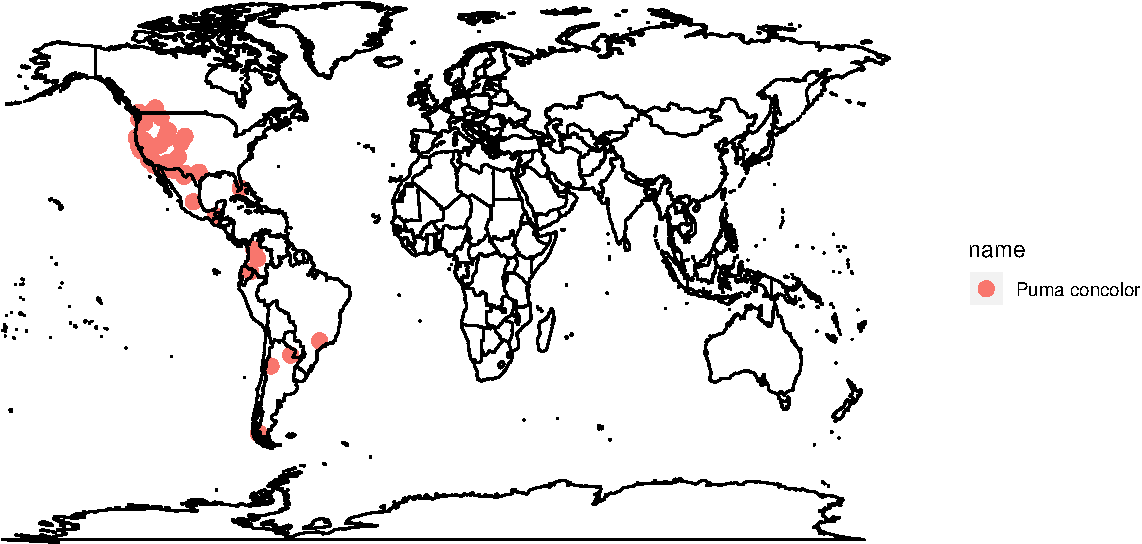
\includegraphics{components/figure/manuscript_mee-unnamed-chunk-47-1.pdf}

\texttt{mapr} has convenient functions for handling input data from
\texttt{rgbif}, \texttt{spocc}, or arbitrary data.frame's, and output
plots for base plots, \texttt{ggplot2}, \texttt{ggmap} (\texttt{ggplot2}
with map layers underneath), and interactive maps on GitHub gists or
with Leaflet.js.

There's no equivalent interface in \texttt{pygbif} or \texttt{gbifrb}.

\hypertarget{citing-gbif-data}{%
\section{Citing GBIF data}\label{citing-gbif-data}}

All the data within GBIF was painstakingly collected by people and
institutions across the globe. They all, including GBIF, deserve to be
cited appropropriately if you use any GBIF data in your research. There
are clear forces making this difficult however. Publishers often limit,
without reason if the publication is online only, the number of
citations one can include a manuscript. Even when this happens, you can
always include additional citations in an appendix.

To make citing data from GBIF easier \texttt{rgbif} has a function
\texttt{gbif\_citation()}, which accepts the output of many different
\texttt{rgbif} functions and gives citations for each dataset
represented in the data therein. For example, suppose you searched for
occurrences for \texttt{taxonKey} 9206251 (\emph{Helianthus annuus}):

\begin{Shaded}
\begin{Highlighting}[]
\NormalTok{res <{-}}\StringTok{ }\KeywordTok{occ\_search}\NormalTok{(}\DataTypeTok{taxonKey =} \DecValTok{9206251}\NormalTok{, }\DataTypeTok{limit =} \DecValTok{20}\NormalTok{)}
\end{Highlighting}
\end{Shaded}

We retrieved 20 occurrences from 4 different datasets.

To get citations for each of the four datasets, one can pass the output
of \texttt{occ\_search()}, here the object \texttt{res}, to the
\texttt{gbif\_citation()} function:

\begin{Shaded}
\begin{Highlighting}[]
\NormalTok{cites <{-}}\StringTok{ }\KeywordTok{gbif\_citation}\NormalTok{(res)}
\NormalTok{cites}
\CommentTok{\#> [[1]]}
\CommentTok{\#> <<rgbif citation>>}
\CommentTok{\#>    Citation: iNaturalist.org (2020). iNaturalist Research{-}grade Observations.}
\CommentTok{\#>         Occurrence dataset https://doi.org/10.15468/ab3s5x accessed via}
\CommentTok{\#>         GBIF.org on 2020{-}02{-}25.. Accessed from R via rgbif}
\CommentTok{\#>         (https://github.com/ropensci/rgbif) on 2020{-}02{-}25}
\CommentTok{\#>    Rights:}
\CommentTok{\#> }
\CommentTok{\#> [[2]]}
\CommentTok{\#> <<rgbif citation>>}
\CommentTok{\#>    Citation: Shah M, Coulson S (2020). Artportalen (Swedish Species Observation}
\CommentTok{\#>         System). Version 92.180. ArtDatabanken. Occurrence dataset}
\CommentTok{\#>         https://doi.org/10.15468/kllkyl accessed via GBIF.org on 2020{-}02{-}25..}
\CommentTok{\#>         Accessed from R via rgbif (https://github.com/ropensci/rgbif) on}
\CommentTok{\#>         2020{-}02{-}25}
\CommentTok{\#>    Rights:}
\CommentTok{\#> }
\CommentTok{\#> [[3]]}
\CommentTok{\#> <<rgbif citation>>}
\CommentTok{\#>    Citation: naturgucker.de. naturgucker. Occurrence dataset}
\CommentTok{\#>         https://doi.org/10.15468/uc1apo accessed via GBIF.org on 2020{-}02{-}25..}
\CommentTok{\#>         Accessed from R via rgbif (https://github.com/ropensci/rgbif) on}
\CommentTok{\#>         2020{-}02{-}25}
\CommentTok{\#>    Rights:}
\CommentTok{\#> }
\CommentTok{\#> [[4]]}
\CommentTok{\#> <<rgbif citation>>}
\CommentTok{\#>    Citation: Vanreusel W, Barendse R, Steeman R, Gielen K, Swinnen K, Desmet P,}
\CommentTok{\#>         Herremans M (2020). Waarnemingen.be {-} Non{-}native plant occurrences in}
\CommentTok{\#>         Flanders and the Brussels Capital Region, Belgium. Version 1.14.}
\CommentTok{\#>         Natuurpunt. Occurrence dataset https://doi.org/10.15468/smdvdo accessed}
\CommentTok{\#>         via GBIF.org on 2020{-}02{-}25.. Accessed from R via rgbif}
\CommentTok{\#>         (https://github.com/ropensci/rgbif) on 2020{-}02{-}25}
\CommentTok{\#>    Rights:}
\end{Highlighting}
\end{Shaded}

And we get four citations, one of each of the datasets behind the 20
occurrence records retrieved.

We don't yet have the same functionality available in \texttt{pygbif},
but it will be coming soon.

\hypertarget{downloads-vs.-searches}{%
\subsection{Downloads vs.~searches}\label{downloads-vs.-searches}}

The distinction between ``downloads'' and ``searches'' is not especially
meaningful with respect to the science done with GBIF data. However,
downloads and searches are different with respect to easily being able
to cite GBIF data, which matters for GBIF and for data providers.

Downloads refers to the \texttt{rgbif} functions that start with
\texttt{occ\_download}, and the \texttt{pygbif} methods that start with
\texttt{occurrences.download}. These methods use the GBIF ``downloads
API'', which you can interact with from \texttt{rgbif} and
\texttt{pygbif} programatically, similar to how you would interact with
the GBIF website - each interaction creating a download request, which
processes in the background. The user has to ask if the request is ready
to download. Downloads can request a very large amount of data.

Searches are faster and more dynamic. Search functions in \texttt{rgbif}
include \texttt{occ\_search}, \texttt{occ\_data}, and \texttt{occ\_get},
while \texttt{pygbif} methods include \texttt{occurrences.search},
\texttt{occurrences.get}. These methods can only request up to 200,000
occurrence records.

The big difference between downloads and searches with respect to
citations is that each download generates a Digital Object Identifier
(or DOI). This DOI can be used cite the entire set of data, that can
inlude many datasets. There's no good way to refer to the entire results
of searches, other than the user manually creating a dataset somewhere
public and linking to it from Zenodo to get a DOI. However, simply using
downloads is simpler in terms of getting a single citeable DOI for the
data used in a research paper/project.

In \texttt{rgbif}, the output of \texttt{occ\_download\_meta()} can be
passed to \texttt{gbif\_citation()} to get the citation for the entire
download.

\begin{Shaded}
\begin{Highlighting}[]
\NormalTok{key <{-}}\StringTok{ "0000122{-}171020152545675"}
\NormalTok{res <{-}}\StringTok{ }\KeywordTok{occ\_download\_meta}\NormalTok{(key)}
\KeywordTok{gbif\_citation}\NormalTok{(res)}
\CommentTok{\#> $download}
\CommentTok{\#> [1] "GBIF Occurrence Download https://doi.org/10.15468/dl.yghxj7 Accessed from R via rgbif (https://github.com/ropensci/rgbif) on 2017{-}10{-}20"}
\CommentTok{\#> }
\CommentTok{\#> $datasets}
\CommentTok{\#> NULL}
\end{Highlighting}
\end{Shaded}

If you however download the data first, then \texttt{gbif\_citation()}
can get citations for all the datasets contained within the download.

\begin{Shaded}
\begin{Highlighting}[]
\NormalTok{d1 <{-}}\StringTok{ }\KeywordTok{occ\_download\_get}\NormalTok{(key, }\DataTypeTok{overwrite =} \OtherTok{TRUE}\NormalTok{)}
\KeywordTok{gbif\_citation}\NormalTok{(d1)}
\CommentTok{\#> $download}
\CommentTok{\#> [1] "GBIF Occurrence Download https://doi.org/10.15468/dl.yghxj7 Accessed from R via rgbif (https://github.com/ropensci/rgbif) on 2017{-}10{-}20"}
\CommentTok{\#> }
\CommentTok{\#> $datasets}
\CommentTok{\#> $datasets[[1]]}
\CommentTok{\#> <<rgbif citation>>}
\CommentTok{\#>    Citation: Grant S, Jones J (2017). Field Museum of Natural History (Zoology)}
\CommentTok{\#>         Invertebrate Collection. Version 18.6. Field Museum. Occurrence Dataset}
\CommentTok{\#>         https://doi.org/10.15468/6q5vuc accessed via GBIF.org on 2017{-}10{-}20..}
\CommentTok{\#>         Accessed from R via rgbif (https://github.com/ropensci/rgbif) on}
\CommentTok{\#>         2020{-}02{-}24}
\CommentTok{\#>    Rights: To the extent possible under law, the publisher has waived all}
\CommentTok{\#>         rights to these data and has dedicated them to the Public Domain (CC0}
\CommentTok{\#>         1.0). Users may copy, modify, distribute and use the work, including}
\CommentTok{\#>         for commercial purposes, without restriction.}
\CommentTok{\#> }
\CommentTok{\#> $datasets[[2]]}
\CommentTok{\#> <<rgbif citation>>}
\CommentTok{\#>    Citation: Creuwels J (2017). Naturalis Biodiversity Center (NL) {-} Crustacea.}
\CommentTok{\#>         Naturalis Biodiversity Center. Occurrence Dataset}
\CommentTok{\#>         https://doi.org/10.15468/vjoltu accessed via GBIF.org on 2017{-}10{-}20..}
\CommentTok{\#>         Accessed from R via rgbif (https://github.com/ropensci/rgbif) on}
\CommentTok{\#>         2020{-}02{-}24}
\CommentTok{\#>    Rights: To the extent possible under law, the publisher has waived all}
\CommentTok{\#>         rights to these data and has dedicated them to the Public Domain (CC0}
\CommentTok{\#>         1.0). Users may copy, modify, distribute and use the work, including}
\CommentTok{\#>         for commercial purposes, without restriction.}
\end{Highlighting}
\end{Shaded}

\hypertarget{gbif-data-in-other-r-packages}{%
\section{GBIF data in other R
packages}\label{gbif-data-in-other-r-packages}}

We discuss usage of GBIF data in other R packages throughout the
manuscript, but provide a synopsis here for clarity.

\hypertarget{taxize}{%
\subsection{taxize}\label{taxize}}

Some of the GBIF taxonomic services are also available in
\href{https://github.com/ropensci/taxize}{taxize}, an R package that
focuses on getting data from taxonomic data sources on the web. For
example, with \texttt{get\_gbifid()} one can get GBIF IDs used for a set
of taxonomic names - then use those IDs in other functions in
\texttt{taxize} to get additional information, like taxonomically
downstream children.

\hypertarget{spocc}{%
\subsection{spocc}\label{spocc}}

GBIF occurrence data is available in the R package
\href{https://github.com/ropensci/spocc}{spocc} via \texttt{rgbif}.
\texttt{spocc} is a unified interface for fetching species occurrence
data from many sources on the web. For example, a user can collect
occurrence data from GBIF, iDigBio, and iNaturalist, and easily combine
them, then use other packages to clean and visualize the data.

\hypertarget{r-vs.-python-vs.-ruby}{%
\section{R vs.~Python vs.~Ruby}\label{r-vs.-python-vs.-ruby}}

Both R and Python are commonly used in science, and can be used for
similar tasks. Python, however, is a more general programming language,
and can be used in more contexts than R can be used in. Ruby is used
very little in science; but, like Python, Ruby is very widely used as a
general purpose programming language, with heavy use in web development
and web services.

The three clients can do a lot of the same tasks. We envision
\texttt{rgbif} being more common in workflows of academics asking
research questions, whereas \texttt{pygbif} and \texttt{gbifrb} can do
that as well, but may be more easily used in a website.

The R client \texttt{rgbif} has had much more development time than
\texttt{pygbif} and \texttt{gbifrb}, but with time \texttt{pygbif} and
\texttt{gbifrb} will become equally mature.

\hypertarget{use-cases}{%
\section{Use cases}\label{use-cases}}

The following are three use cases for the R library \texttt{rgbif}:
niche modeling, spatial change in biodiversity, and distribution
mapping.

\hypertarget{ecological-niche-modeling}{%
\subsection{Ecological niche modeling}\label{ecological-niche-modeling}}

In this example, we plot actual occurrence data for \emph{Bradypus}
species against a single predictor variable, BIO1 (annual mean
temperature). This is only one step in a species distribution modelling
workflow.

This example can be done using BISON data as well with our rbison
package.

\emph{Load libraries}

\begin{Shaded}
\begin{Highlighting}[]
\KeywordTok{library}\NormalTok{(}\StringTok{"sp"}\NormalTok{)}
\KeywordTok{library}\NormalTok{(}\StringTok{"rgbif"}\NormalTok{)}
\KeywordTok{library}\NormalTok{(}\StringTok{"dismo"}\NormalTok{)}
\KeywordTok{library}\NormalTok{(}\StringTok{"maptools"}\NormalTok{)}
\KeywordTok{library}\NormalTok{(}\StringTok{"dplyr"}\NormalTok{)}
\end{Highlighting}
\end{Shaded}

\emph{Raster files}

Make a list of files that are installed with the dismo package, then
create a rasterStack from these

\begin{Shaded}
\begin{Highlighting}[]
\NormalTok{files <{-}}\StringTok{ }\KeywordTok{list.files}\NormalTok{(}\KeywordTok{paste}\NormalTok{(}\KeywordTok{system.file}\NormalTok{(}\DataTypeTok{package =} \StringTok{"dismo"}\NormalTok{), }\StringTok{"/ex"}\NormalTok{, }\DataTypeTok{sep =} \StringTok{""}\NormalTok{),}
                    \StringTok{"grd"}\NormalTok{, }\DataTypeTok{full.names =} \OtherTok{TRUE}\NormalTok{)}
\NormalTok{predictors <{-}}\StringTok{ }\KeywordTok{stack}\NormalTok{(files)}
\end{Highlighting}
\end{Shaded}

\emph{Get world boundaries}

\begin{Shaded}
\begin{Highlighting}[]
\KeywordTok{data}\NormalTok{(wrld\_simpl)}
\end{Highlighting}
\end{Shaded}

\emph{Get GBIF data using the rOpenSci package rgbif}

\begin{Shaded}
\begin{Highlighting}[]
\NormalTok{nn <{-}}\StringTok{ }\KeywordTok{name\_lookup}\NormalTok{(}\StringTok{"bradypus*"}\NormalTok{, }\DataTypeTok{rank =} \StringTok{"species"}\NormalTok{)}
\NormalTok{nn <{-}}\StringTok{ }\KeywordTok{na.omit}\NormalTok{(}\KeywordTok{unique}\NormalTok{(nn}\OperatorTok{$}\NormalTok{data}\OperatorTok{$}\NormalTok{nubKey))}
\NormalTok{df <{-}}\StringTok{ }\KeywordTok{occ\_search}\NormalTok{(}\DataTypeTok{taxonKey =}\NormalTok{ nn, }\DataTypeTok{hasCoordinate =} \OtherTok{TRUE}\NormalTok{, }\DataTypeTok{limit =} \DecValTok{500}\NormalTok{)}
\NormalTok{df\_data <{-}}\StringTok{ }\NormalTok{df[ }\KeywordTok{sapply}\NormalTok{(df, }\ControlFlowTok{function}\NormalTok{(x) }\KeywordTok{any}\NormalTok{(}\KeywordTok{class}\NormalTok{(x}\OperatorTok{$}\NormalTok{data) }\OperatorTok{\%in\%}\StringTok{ "tbl\_df"}\NormalTok{)) ]}
\NormalTok{df\_data <{-}}\StringTok{ }\NormalTok{dplyr}\OperatorTok{::}\KeywordTok{bind\_rows}\NormalTok{(}\KeywordTok{lapply}\NormalTok{(df\_data, }\StringTok{"[["}\NormalTok{, }\StringTok{"data"}\NormalTok{))}
\NormalTok{df2 <{-}}\StringTok{ }\NormalTok{df\_data }\OperatorTok{\%>\%}\StringTok{ }\NormalTok{dplyr}\OperatorTok{::}\KeywordTok{select}\NormalTok{(decimalLongitude, decimalLatitude)}
\end{Highlighting}
\end{Shaded}

\emph{Plot}

\begin{enumerate}
\def\labelenumi{(\arabic{enumi})}
\tightlist
\item
  Add raster data, (2) Add political boundaries, (3) Add the points
  (occurrences)
\end{enumerate}

\begin{Shaded}
\begin{Highlighting}[]
\KeywordTok{plot}\NormalTok{(predictors, }\DecValTok{1}\NormalTok{)}
\KeywordTok{plot}\NormalTok{(wrld\_simpl, }\DataTypeTok{add =} \OtherTok{TRUE}\NormalTok{)}
\KeywordTok{points}\NormalTok{(df2, }\DataTypeTok{col =} \StringTok{"blue"}\NormalTok{)}
\end{Highlighting}
\end{Shaded}

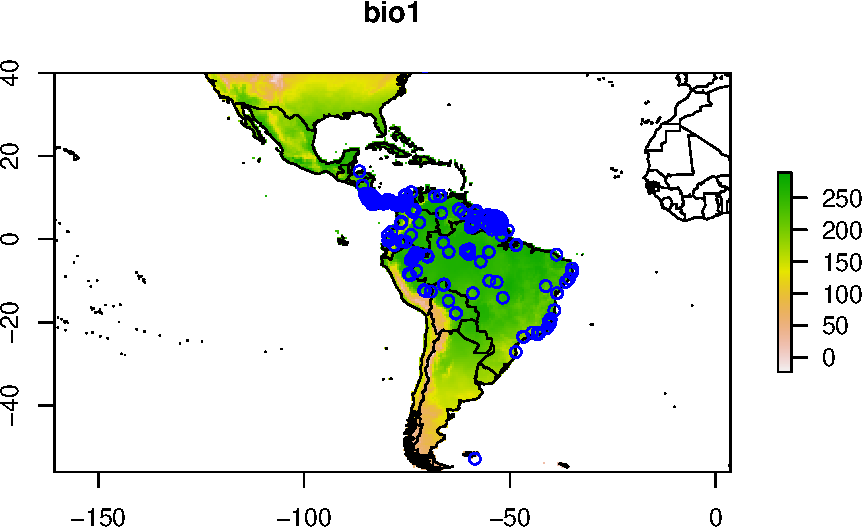
\includegraphics{components/figure/manuscript_mee-unnamed-chunk-57-1.pdf}

\hypertarget{biodiversity-in-big-cities}{%
\subsection{Biodiversity in big
cities}\label{biodiversity-in-big-cities}}

In this example, we collect specimen records across different cities
using GBIF data from the \texttt{rgbif} package.

\emph{Load libraries}

\begin{Shaded}
\begin{Highlighting}[]
\KeywordTok{library}\NormalTok{(}\StringTok{"rgbif"}\NormalTok{)}
\KeywordTok{library}\NormalTok{(}\StringTok{"ggplot2"}\NormalTok{)}
\KeywordTok{library}\NormalTok{(}\StringTok{"plyr"}\NormalTok{)}
\KeywordTok{library}\NormalTok{(}\StringTok{"httr"}\NormalTok{)}
\KeywordTok{library}\NormalTok{(}\StringTok{"RColorBrewer"}\NormalTok{)}
\KeywordTok{library}\NormalTok{(}\StringTok{"wicket"}\NormalTok{)}
\end{Highlighting}
\end{Shaded}

\emph{Get bounding boxes for some cites}

Bounding lat/long data is from
\url{https://raw.github.com/amyxzhang/boundingbox-cities/master/boundbox.txt}.

\begin{Shaded}
\begin{Highlighting}[]
\NormalTok{url <{-}}\StringTok{ \textquotesingle{}https://raw.githubusercontent.com/amyxzhang/}
\StringTok{boundingbox{-}cities/master/boundbox.txt\textquotesingle{}}
\NormalTok{rawdat <{-}}\StringTok{ }\KeywordTok{content}\NormalTok{(}\KeywordTok{GET}\NormalTok{(}\KeywordTok{sub}\NormalTok{(}\StringTok{"}\CharTok{\textbackslash{}n}\StringTok{"}\NormalTok{, }\StringTok{""}\NormalTok{, url)), }\DataTypeTok{as =} \StringTok{"text"}\NormalTok{)}
\NormalTok{dat <{-}}\StringTok{ }\KeywordTok{read.table}\NormalTok{(}
  \DataTypeTok{text =}\NormalTok{ rawdat, }\DataTypeTok{header =} \OtherTok{FALSE}\NormalTok{,}
  \DataTypeTok{sep =} \StringTok{"}\CharTok{\textbackslash{}t}\StringTok{"}\NormalTok{, }\DataTypeTok{col.names =} \KeywordTok{c}\NormalTok{(}\StringTok{"city"}\NormalTok{,}\StringTok{"minlat"}\NormalTok{,}\StringTok{"maxlon"}\NormalTok{,}\StringTok{"maxlat"}\NormalTok{,}\StringTok{"minlon"}\NormalTok{),}
  \DataTypeTok{stringsAsFactors =} \OtherTok{FALSE}\NormalTok{)}
\NormalTok{dat <{-}}\StringTok{ }\KeywordTok{data.frame}\NormalTok{(}
  \DataTypeTok{city =}\NormalTok{ dat}\OperatorTok{$}\NormalTok{city, }\DataTypeTok{minlon =}\NormalTok{ dat}\OperatorTok{$}\NormalTok{minlon,}
  \DataTypeTok{minlat =}\NormalTok{ dat}\OperatorTok{$}\NormalTok{minlat, }\DataTypeTok{maxlon =}\NormalTok{ dat}\OperatorTok{$}\NormalTok{maxlon,}
  \DataTypeTok{maxlat =}\NormalTok{ dat}\OperatorTok{$}\NormalTok{maxlat,}
  \DataTypeTok{stringsAsFactors =} \OtherTok{FALSE}
\NormalTok{)}
\end{Highlighting}
\end{Shaded}

A helper function to get count data. GBIF has a count API, but we can't
use that with a geometry search as that API doesn't support geospatial
search. We can however use the search API via \texttt{occ\_search()} and
set \texttt{limit\ =\ 1} so that we

\begin{Shaded}
\begin{Highlighting}[]
\NormalTok{getdata <{-}}\StringTok{ }\ControlFlowTok{function}\NormalTok{(x)\{}
\NormalTok{  coords <{-}}\StringTok{ }\KeywordTok{as.numeric}\NormalTok{(x[}\KeywordTok{c}\NormalTok{(}\StringTok{\textquotesingle{}minlon\textquotesingle{}}\NormalTok{,}\StringTok{\textquotesingle{}minlat\textquotesingle{}}\NormalTok{,}\StringTok{\textquotesingle{}maxlon\textquotesingle{}}\NormalTok{,}\StringTok{\textquotesingle{}maxlat\textquotesingle{}}\NormalTok{)])}
\NormalTok{  wkt <{-}}\StringTok{ }\NormalTok{wicket}\OperatorTok{::}\KeywordTok{wkt\_correct}\NormalTok{(wicket}\OperatorTok{::}\KeywordTok{bounding\_wkt}\NormalTok{(}\DataTypeTok{values =}\NormalTok{ coords))}
\NormalTok{  num <{-}}\StringTok{ }\KeywordTok{occ\_search}\NormalTok{(}\DataTypeTok{geometry =}\NormalTok{ wkt, }\DataTypeTok{limit =} \DecValTok{1}\NormalTok{)}\OperatorTok{$}\NormalTok{meta}\OperatorTok{$}\NormalTok{count}
  \KeywordTok{data.frame}\NormalTok{(}
    \DataTypeTok{city =}\NormalTok{ x[}\StringTok{\textquotesingle{}city\textquotesingle{}}\NormalTok{],}
    \DataTypeTok{richness =}\NormalTok{ num,}
    \DataTypeTok{stringsAsFactors =} \OtherTok{FALSE}
\NormalTok{  )}
\NormalTok{\}}
\end{Highlighting}
\end{Shaded}

\begin{Shaded}
\begin{Highlighting}[]
\NormalTok{out <{-}}\StringTok{ }\KeywordTok{apply}\NormalTok{(dat, }\DecValTok{1}\NormalTok{, getdata)}
\end{Highlighting}
\end{Shaded}

\emph{Merge to original table}

\begin{Shaded}
\begin{Highlighting}[]
\NormalTok{out <{-}}\StringTok{ }\KeywordTok{merge}\NormalTok{(dat, }\KeywordTok{ldply}\NormalTok{(out), }\DataTypeTok{by =} \StringTok{"city"}\NormalTok{)}
\end{Highlighting}
\end{Shaded}

\emph{Add centroids from bounding boxes}

\begin{Shaded}
\begin{Highlighting}[]
\NormalTok{out <{-}}\StringTok{ }\KeywordTok{transform}\NormalTok{(out, }\DataTypeTok{lat =}\NormalTok{ (minlat }\OperatorTok{+}\StringTok{ }\NormalTok{maxlat)}\OperatorTok{/}\DecValTok{2}\NormalTok{, }\DataTypeTok{lon =}\NormalTok{ (minlon }\OperatorTok{+}\StringTok{ }\NormalTok{maxlon)}\OperatorTok{/}\DecValTok{2}\NormalTok{)}
\end{Highlighting}
\end{Shaded}

\emph{Plot data}

\begin{Shaded}
\begin{Highlighting}[]
\NormalTok{mapp <{-}}\StringTok{ }\KeywordTok{map\_data}\NormalTok{(}\StringTok{\textquotesingle{}world\textquotesingle{}}\NormalTok{)}
\KeywordTok{ggplot}\NormalTok{(mapp, }\KeywordTok{aes}\NormalTok{(long, lat)) }\OperatorTok{+}
\StringTok{  }\KeywordTok{geom\_polygon}\NormalTok{(}\KeywordTok{aes}\NormalTok{(}\DataTypeTok{group=}\NormalTok{group), }\DataTypeTok{fill=}\StringTok{"white"}\NormalTok{, }\DataTypeTok{alpha=}\DecValTok{0}\NormalTok{, }\DataTypeTok{color=}\StringTok{"black"}\NormalTok{, }\DataTypeTok{size=}\FloatTok{0.4}\NormalTok{) }\OperatorTok{+}
\StringTok{  }\KeywordTok{geom\_point}\NormalTok{(}\DataTypeTok{data=}\NormalTok{out, }\KeywordTok{aes}\NormalTok{(lon, lat, }\DataTypeTok{color=}\NormalTok{richness), }\DataTypeTok{size=}\DecValTok{5}\NormalTok{, }\DataTypeTok{alpha=}\FloatTok{0.8}\NormalTok{) }\OperatorTok{+}
\StringTok{  }\KeywordTok{scale\_color\_continuous}\NormalTok{(}\DataTypeTok{low =} \StringTok{"\#60E1EE"}\NormalTok{, }\DataTypeTok{high =} \StringTok{"\#0404C8"}\NormalTok{) }\OperatorTok{+}
\StringTok{  }\KeywordTok{labs}\NormalTok{(}\DataTypeTok{x=}\StringTok{""}\NormalTok{, }\DataTypeTok{y=}\StringTok{""}\NormalTok{) }\OperatorTok{+}
\StringTok{  }\KeywordTok{theme\_grey}\NormalTok{(}\DataTypeTok{base\_size=}\DecValTok{14}\NormalTok{) }\OperatorTok{+}
\StringTok{  }\KeywordTok{theme}\NormalTok{(}\DataTypeTok{legend.position =} \StringTok{"bottom"}\NormalTok{, }\DataTypeTok{legend.key =} \KeywordTok{element\_blank}\NormalTok{()) }\OperatorTok{+}
\StringTok{  }\KeywordTok{guides}\NormalTok{(}\DataTypeTok{color =} \KeywordTok{guide\_legend}\NormalTok{(}\DataTypeTok{keywidth =} \DecValTok{2}\NormalTok{))}
\end{Highlighting}
\end{Shaded}

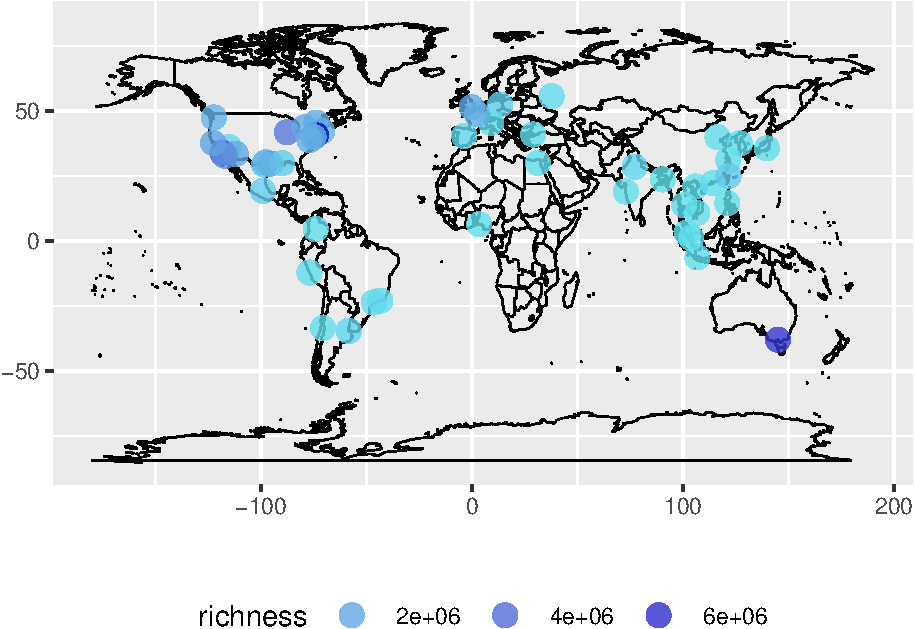
\includegraphics{components/figure/manuscript_mee-unnamed-chunk-62-1.pdf}

\hypertarget{valley-oak-occurrence-data-comparison}{%
\subsection{Valley oak occurrence data
comparison}\label{valley-oak-occurrence-data-comparison}}

This example is inspired by a tweet from
\href{https://twitter.com/ajpelu}{Antonio J. Perez-Luque} who
\href{https://twitter.com/ajpelu/status/473951167567757312}{shared his
plot on Twitter}. Antonio compared the occurrences of Valley Oak
(\emph{Quercus lobata}) from \href{http://www.gbif.org/}{GBIF} to the
distribution of the same species from the
\href{http://esp.cr.usgs.gov/data/little/}{Atlas of US Trees}.

The data in question from the example above is no longer available, so
below we use a different species.

\emph{Load libraries}

\begin{Shaded}
\begin{Highlighting}[]
\KeywordTok{library}\NormalTok{(}\StringTok{\textquotesingle{}rgbif\textquotesingle{}}\NormalTok{)}
\KeywordTok{library}\NormalTok{(}\StringTok{\textquotesingle{}raster\textquotesingle{}}\NormalTok{)}
\KeywordTok{library}\NormalTok{(}\StringTok{\textquotesingle{}sp\textquotesingle{}}\NormalTok{)}
\KeywordTok{library}\NormalTok{(}\StringTok{\textquotesingle{}sf\textquotesingle{}}\NormalTok{)}
\KeywordTok{library}\NormalTok{(}\StringTok{\textquotesingle{}rgeos\textquotesingle{}}\NormalTok{)}
\KeywordTok{library}\NormalTok{(}\StringTok{\textquotesingle{}scales\textquotesingle{}}\NormalTok{)}
\KeywordTok{library}\NormalTok{(}\StringTok{\textquotesingle{}rnaturalearth\textquotesingle{}}\NormalTok{)}
\end{Highlighting}
\end{Shaded}

\emph{Get GBIF Data for Fraxinus excelsior}

\begin{Shaded}
\begin{Highlighting}[]
\NormalTok{keyFe <{-}}\StringTok{ }\KeywordTok{name\_backbone}\NormalTok{(}\DataTypeTok{name =} \StringTok{\textquotesingle{}Fraxinus excelsior\textquotesingle{}}\NormalTok{, }\DataTypeTok{kingdom =} \StringTok{\textquotesingle{}plants\textquotesingle{}}\NormalTok{)}\OperatorTok{$}\NormalTok{speciesKey}
\NormalTok{dat.Fe <{-}}\StringTok{ }\KeywordTok{occ\_search}\NormalTok{(}\DataTypeTok{taxonKey =}\NormalTok{ keyFe, }\DataTypeTok{return =} \StringTok{\textquotesingle{}data\textquotesingle{}}\NormalTok{, }\DataTypeTok{limit =}\NormalTok{ 10000L)}
\end{Highlighting}
\end{Shaded}

\emph{Get Distribution map of F. excelsior European Forest Genetic
Resources Programme}

From \url{http://www.euforgen.org/species/fraxinus-excelsior/}. And save
shapefile in same directory

\begin{Shaded}
\begin{Highlighting}[]
\NormalTok{url <{-}}\StringTok{ \textquotesingle{}http://www.euforgen.org/fileadmin/templates/euforgen.org/upload/Documents/Maps/Shapefile/Fraxinus\_excelsior.zip\textquotesingle{}}
\NormalTok{tmp <{-}}\StringTok{ }\KeywordTok{tempdir}\NormalTok{()}
\KeywordTok{download.file}\NormalTok{(url, }\DataTypeTok{destfile =} \StringTok{"fraxinus\_excelsior.zip"}\NormalTok{)}
\KeywordTok{unzip}\NormalTok{(}\StringTok{"fraxinus\_excelsior.zip"}\NormalTok{, }\DataTypeTok{exdir =}\NormalTok{ tmp)}
\NormalTok{fe <{-}}\StringTok{ }\NormalTok{sf}\OperatorTok{::}\KeywordTok{read\_sf}\NormalTok{(}\KeywordTok{file.path}\NormalTok{(tmp, }\StringTok{"Fraxinus\_excelsior\_EUFORGEN.shp"}\NormalTok{))}
\end{Highlighting}
\end{Shaded}

\emph{Get Elevation data of US}

\begin{Shaded}
\begin{Highlighting}[]
\NormalTok{eur <{-}}\StringTok{ }\NormalTok{rnaturalearth}\OperatorTok{::}\KeywordTok{ne\_countries}\NormalTok{(}\DataTypeTok{continent =} \StringTok{"europe"}\NormalTok{, }\DataTypeTok{type =} \StringTok{"map\_units"}\NormalTok{)}
\NormalTok{eur1 <{-}}\StringTok{ }\NormalTok{eur[eur}\OperatorTok{$}\NormalTok{sovereignt }\OperatorTok{!=}\StringTok{ "Russia"}\NormalTok{, ]}
\end{Highlighting}
\end{Shaded}

\emph{Plot map}

\begin{Shaded}
\begin{Highlighting}[]
\KeywordTok{plot}\NormalTok{(eur1, }\DataTypeTok{col =} \StringTok{"darkgrey"}\NormalTok{, }\DataTypeTok{legend =} \OtherTok{FALSE}\NormalTok{,}
     \DataTypeTok{main =} \StringTok{\textquotesingle{}Distribution of Fraxinus excelsior\textquotesingle{}}\NormalTok{)}
\CommentTok{\# add distribution range layer}
\KeywordTok{plot}\NormalTok{(fe, }\DataTypeTok{add =} \OtherTok{TRUE}\NormalTok{, }\DataTypeTok{col =} \KeywordTok{alpha}\NormalTok{(}\StringTok{"white"}\NormalTok{, }\FloatTok{0.5}\NormalTok{), }\DataTypeTok{border =} \OtherTok{FALSE}\NormalTok{)}
\CommentTok{\# add Gbif presence points}
\KeywordTok{points}\NormalTok{(dat.Fe}\OperatorTok{$}\NormalTok{decimalLongitude, dat.Fe}\OperatorTok{$}\NormalTok{decimalLatitude,}
       \DataTypeTok{cex =} \FloatTok{.7}\NormalTok{, }\DataTypeTok{pch =} \DecValTok{19}\NormalTok{, }\DataTypeTok{col =} \KeywordTok{alpha}\NormalTok{(}\StringTok{"darkgreen"}\NormalTok{, }\FloatTok{0.8}\NormalTok{))}
\KeywordTok{legend}\NormalTok{(}\DataTypeTok{x =} \DecValTok{38}\NormalTok{, }\DataTypeTok{y =} \DecValTok{81}\NormalTok{, }\KeywordTok{c}\NormalTok{(}\StringTok{"GBIF Data"}\NormalTok{, }\StringTok{"Range Layer"}\NormalTok{), }\DataTypeTok{pch =} \DecValTok{19}\NormalTok{, }\DataTypeTok{bg =} \StringTok{"grey"}\NormalTok{,}
       \DataTypeTok{col =} \KeywordTok{c}\NormalTok{(}\StringTok{\textquotesingle{}darkgreen\textquotesingle{}}\NormalTok{, }\KeywordTok{alpha}\NormalTok{(}\StringTok{"white"}\NormalTok{, }\FloatTok{0.5}\NormalTok{)), }\DataTypeTok{pt.cex =} \DecValTok{1}\NormalTok{, }\DataTypeTok{cex =} \FloatTok{.8}\NormalTok{)}
\end{Highlighting}
\end{Shaded}

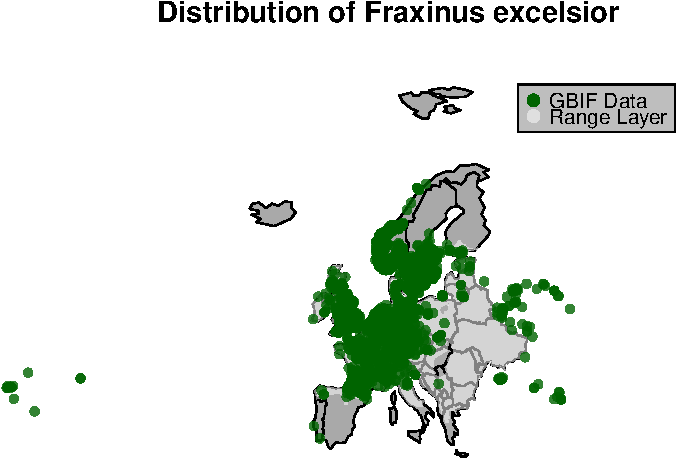
\includegraphics{components/figure/manuscript_mee-unnamed-chunk-68-1.pdf}

\hypertarget{conclusions-and-future-directions}{%
\section{Conclusions and future
directions}\label{conclusions-and-future-directions}}

The \texttt{rgbif}, \texttt{pygbif}, and \texttt{gbibrb} libraries
provide programmatic interfaces to GBIF's application programming
interface (API) - a powerful tool for working with species occurrence
data, and facilitating reproducible research. In fact, the
\texttt{rgbif} package has already been used in more than 20 scholarly
publications (as of 2020-02-25), including (Drozd \& Šipoš 2013;
Bartomeus \emph{et al.} 2013; Barve 2014; Richardson \emph{et al.} 2015;
Feitosa \emph{et al.} 2015; Collins \emph{et al.} 2015; Malhado \emph{et
al.} 2015; Kong \emph{et al.} 2015; Werner \emph{et al.} 2015; Bone
\emph{et al.} 2015; Turner \emph{et al.} 2015; Davison \emph{et al.}
2015; Verheijen \emph{et al.} 2015; Dellinger \emph{et al.} 2015; Zizka
\& Antonelli 2015; Janssens \emph{et al.} 2016; Robertson \emph{et al.}
2016; Amano \emph{et al.} 2016; Butterfield \emph{et al.} 2016).

The \texttt{rgbif} package is stable, and should not have many breaking
changes unless necessitated due to changes in the GBIF API. The
\texttt{pygbif} and \texttt{gbifrb} libraries are in early development,
and will greatly benefit from any feedback and use cases.

One area of focus in the future is to attempt to solve many use cases
that have been brought up with respect to GBIF data. For example, some
specimens are included in GBIF that are located in botanical gardens.
For many research questions, researchers are interested in ``wild'' type
occurrences, not those in human curated scenarios. Making removal of
these occurrences easy would be very useful, but is actually quite a
hard problem. There are many other problems like this, for which these
three libraries will help in making more efficient and reproducible.

\hypertarget{acknowledgments}{%
\section{Acknowledgments}\label{acknowledgments}}

This project was supported in part by the Alfred P Sloan Foundation
(Grant No.~G-2014-13485), and in part by the Helmsley Foundation (Grant
No.~2016PG-BRI004).

\hypertarget{data-accessibility}{%
\section{Data Accessibility}\label{data-accessibility}}

All scripts and data used in this paper can be found in the permanent
data archive Zenodo under the digital object identifier
(\url{https://doi.org/10.5281/zenodo.997554}). This DOI corresponds to a
snapshot of the GitHub repository at
\url{https://github.com/sckott/gbifms} that matches this preprint.
Software can be found at \url{https://github.com/ropensci/rgbif},
\url{https://github.com/sckott/pygbif}, and
\url{https://github.com/sckott/gibfrb}, all under MIT licenses. We thank
all the users that have used \texttt{rgbif}, \texttt{pygbif}, and
\texttt{gbifrb} and have given feedback and reported bugs. In addition,
we greatly appreciate all the contributors to the three libraries, found
at \url{https://github.com/ropensci/rgbif/graphs/contributors},
\url{https://github.com/sckott/pygbif/graphs/contributors}, and
\url{https://github.com/sckott/gbifrb/graphs/contributors}.

\hypertarget{references}{%
\section*{References}\label{references}}
\addcontentsline{toc}{section}{References}

\hypertarget{refs}{}
\begin{cslreferences}
\leavevmode\hypertarget{ref-Amano_2016}{}%
Amano, T., Lamming, J.D.L. \& Sutherland, W.J. (2016). Spatial gaps in
global biodiversity information and the role of citizen science.
\emph{BioScience}, \textbf{66}, 393--400. Retrieved from
\url{http://dx.doi.org/10.1093/biosci/biw022}

\leavevmode\hypertarget{ref-Bartomeus_2013}{}%
Bartomeus, I., Park, M.G., Gibbs, J., Danforth, B.N., Lakso, A.N. \&
Winfree, R. (2013). Biodiversity ensures plant-pollinator phenological
synchrony against climate change (M. Eubanks, Ed.). \emph{Ecology
Letters}, \textbf{16}, 1331--1338. Retrieved from
\url{http://dx.doi.org/10.1111/ele.12170}

\leavevmode\hypertarget{ref-Barve_2014}{}%
Barve, V. (2014). Discovering and developing primary biodiversity data
from social networking sites: A novel approach. \emph{Ecological
Informatics}, \textbf{24}, 194--199. Retrieved from
\url{http://dx.doi.org/10.1016/j.ecoinf.2014.08.008}

\leavevmode\hypertarget{ref-Beck_2012}{}%
Beck, J., Ballesteros-Mejia, L., Buchmann, C.M., Dengler, J., Fritz,
S.A., Gruber, B., Hof, C., Jansen, F., Knapp, S., Kreft, H., Schneider,
A.-K., Winter, M. \& Dormann, C.F. (2012). Whats on the horizon for
macroecology? \emph{Ecography}, \textbf{35}, 673--683. Retrieved from
\url{http://dx.doi.org/10.1111/j.1600-0587.2012.07364.x}

\leavevmode\hypertarget{ref-Bone_2015}{}%
Bone, R.E., Smith, J.A.C., Arrigo, N. \& Buerki, S. (2015). A
macro-ecological perspective on crassulacean acid metabolism (CAM)
photosynthesis evolution in afro-madagascan drylands: Eulophiinae
orchids as a case study. \emph{New Phytologist}, \textbf{208}, 469--481.
Retrieved from \url{http://dx.doi.org/10.1111/nph.13572}

\leavevmode\hypertarget{ref-Brown_1995}{}%
Brown, J.H. (1995). \emph{Macroecology}. University of Chicago Press.

\leavevmode\hypertarget{ref-Brown_2015}{}%
Brown, K.A., Parks, K.E., Bethell, C.A., Johnson, S.E. \& Mulligan, M.
(2015). Predicting plant diversity patterns in madagascar: Understanding
the effects of climate and land cover change in a biodiversity hotspot
(L. Kumar, Ed.). \emph{PLOS ONE}, \textbf{10}, e0122721. Retrieved from
\url{http://dx.doi.org/10.1371/journal.pone.0122721}

\leavevmode\hypertarget{ref-Butterfield_2016}{}%
Butterfield, B.J., Copeland, S.M., Munson, S.M., Roybal, C.M. \& Wood,
T.E. (2016). Prestoration: Using species in restoration that will
persist now and into the future. \emph{Restor Ecol}. Retrieved from
\url{http://dx.doi.org/10.1111/rec.12381}

\leavevmode\hypertarget{ref-Ceballos_2015}{}%
Ceballos, G., Ehrlich, P.R., Barnosky, A.D., Garcia, A., Pringle, R.M.
\& Palmer, T.M. (2015). Accelerated modern human-induced species losses:
Entering the sixth mass extinction. \emph{Science Advances}, \textbf{1},
e1400253--e1400253. Retrieved from
\url{http://dx.doi.org/10.1126/sciadv.1400253}

\leavevmode\hypertarget{ref-gbifrb}{}%
Chamberlain, S. \emph{gbifrb: A ruby interface to the global
biodiversity information facility API}. Retrieved from
\url{https://github.com/sckott/gbifrb}

\leavevmode\hypertarget{ref-pygbif}{}%
Chamberlain, S. \emph{pygbif: A python interface to the global
biodiversity information facility API}. Retrieved from
\url{https://github.com/sckott/pygbif}

\leavevmode\hypertarget{ref-rgbif}{}%
Chamberlain, S., Ram, K., Barve, V. \& Mcglinn, D. \emph{rgbif: An r
interface to the global 'biodiversity' information facility API}.
Retrieved from \url{https://github.com/ropensci/rgbif}

\leavevmode\hypertarget{ref-Collins_2015}{}%
Collins, R., Ribeiro, E.D., Machado, V.N., Hrbek, T. \& Farias, I.
(2015). A preliminary inventory of the catfishes of the lower rio
nhamundá, brazil (ostariophysi, siluriformes). \emph{BDJ}, \textbf{3},
e4162. Retrieved from \url{http://dx.doi.org/10.3897/bdj.3.e4162}

\leavevmode\hypertarget{ref-Davison_2015}{}%
Davison, J., Moora, M., Opik, M., Adholeya, A., Ainsaar, L., Ba, A.,
Burla, S., Diedhiou, A.G., Hiiesalu, I., Jairus, T., Johnson, N.C.,
Kane, A., Koorem, K., Kochar, M., Ndiaye, C., Partel, M., Reier, U.,
Saks, U., Singh, R., Vasar, M. \& Zobel, M. (2015). Global assessment of
arbuscular mycorrhizal fungus diversity reveals very low endemism.
\emph{Science}, \textbf{349}, 970--973. Retrieved from
\url{http://dx.doi.org/10.1126/science.aab1161}

\leavevmode\hypertarget{ref-Dellinger_2015}{}%
Dellinger, A.S., Essl, F., Hojsgaard, D., Kirchheimer, B., Klatt, S.,
Dawson, W., Pergl, J., Pyšek, P., Kleunen, M. van, Weber, E., Winter,
M., Hörandl, E. \& Dullinger, S. (2015). Niche dynamics of alien species
do not differ among sexual and apomictic flowering plants. \emph{New
Phytologist}, \textbf{209}, 1313--1323. Retrieved from
\url{http://dx.doi.org/10.1111/nph.13694}

\leavevmode\hypertarget{ref-Drozd_2013}{}%
Drozd, P. \& Šipoš, J. (2013). R for all (i): Introduction to the new
age of biological analyses. \emph{Casopis slezskeho zemskeho muzea (A)},
\textbf{62}. Retrieved from
\url{http://dx.doi.org/10.2478/cszma-2013-0004}

\leavevmode\hypertarget{ref-Faulkner_2014}{}%
Faulkner, K.T., Robertson, M.P., Rouget, M. \& Wilson, J.R.U. (2014). A
simple, rapid methodology for developing invasive species watch lists.
\emph{Biological Conservation}, \textbf{179}, 25--32. Retrieved from
\url{http://dx.doi.org/10.1016/j.biocon.2014.08.014}

\leavevmode\hypertarget{ref-Di_Febbraro_2013}{}%
Febbraro, M.D., Lurz, P.W.W., Genovesi, P., Maiorano, L., Girardello, M.
\& Bertolino, S. (2013). The use of climatic niches in screening
procedures for introduced species to evaluate risk of spread: A case
with the american eastern grey squirrel (H. Verbruggen, Ed.). \emph{PLoS
ONE}, \textbf{8}, e66559. Retrieved from
\url{http://dx.doi.org/10.1371/journal.pone.0066559}

\leavevmode\hypertarget{ref-Feitosa_2015}{}%
Feitosa, Y.O., Absy, M.L., Latrubesse, E.M. \& Stevaux, J.C. (2015).
Late quaternary vegetation dynamics from central parts of the madeira
river in brazil. \emph{Acta Bot. Bras.}, \textbf{29}, 120--128.
Retrieved from \url{http://dx.doi.org/10.1590/0102-33062014abb3711}

\leavevmode\hypertarget{ref-Ferretti_2015}{}%
Ferretti, F., Verd, G.M., Seret, B., Šprem, J.S. \& Micheli, F. (2015).
Falling through the cracks: The fading history of a large iconic
predator. \emph{Fish and Fisheries}, n/a--n/a. Retrieved from
\url{http://dx.doi.org/10.1111/faf.12108}

\leavevmode\hypertarget{ref-Ficetola_2014}{}%
Ficetola, G.F., Rondinini, C., Bonardi, A., Baisero, D. \&
Padoa-Schioppa, E. (2014). Habitat availability for amphibians and
extinction threat: A global analysis (D. Richardson, Ed.).
\emph{Diversity and Distributions}, \textbf{21}, 302--311. Retrieved
from \url{http://dx.doi.org/10.1111/ddi.12296}

\leavevmode\hypertarget{ref-wkt}{}%
Herring, J. (2011). OpenGIS implementation standard for geographic
information-simple feature access-part 1: Common architecture. \emph{OGC
Document}, \textbf{4}, 122--127. Retrieved from
\url{http://www.opengeospatial.org/standards/sfa}

\leavevmode\hypertarget{ref-Janssens_2016}{}%
Janssens, S.B., Vandelook, F., Langhe, E.D., Verstraete, B., Smets, E.,
Vandenhouwe, I. \& Swennen, R. (2016). Evolutionary dynamics and
biogeography of musaceae reveal a correlation between the
diversification of the banana family and the geological and climatic
history of southeast asia. \emph{New Phytologist}, \textbf{210},
1453--1465. Retrieved from \url{http://dx.doi.org/10.1111/nph.13856}

\leavevmode\hypertarget{ref-Kong_2015}{}%
Kong, X., Huang, M. \& Duan, R. (2015). SDMdata: A web-based software
tool for collecting species occurrence records (J.H. Badger, Ed.).
\emph{PLOS ONE}, \textbf{10}, e0128295. Retrieved from
\url{http://dx.doi.org/10.1371/journal.pone.0128295}

\leavevmode\hypertarget{ref-Malhado_2015}{}%
Malhado, A.C.M., Oliveira-Neto, J.A., Stropp, J., Strona, G., Dias,
L.C.P., Pinto, L.B. \& Ladle, R.J. (2015). Climatological correlates of
seed size in amazonian forest trees (T. Nakashizuka, Ed.). \emph{J Veg
Sci}, \textbf{26}, 956--963. Retrieved from
\url{http://dx.doi.org/10.1111/jvs.12301}

\leavevmode\hypertarget{ref-Mendoza_2015}{}%
Marı́a Mendoza, Ospina, O.E., Cárdenas-Henao, H. \& Garcı́a-R, J.C.
(2015). A likelihood inference of historical biogeography in the world's
most diverse terrestrial vertebrate genus: Diversification of
direct-developing frogs (craugastoridae: Pristimantis) across the
neotropics. \emph{Molecular Phylogenetics and Evolution}, \textbf{85},
50--58. Retrieved from
\url{http://dx.doi.org/10.1016/j.ympev.2015.02.001}

\leavevmode\hypertarget{ref-Pimm_2014}{}%
Pimm, S.L., Jenkins, C.N., Abell, R., Brooks, T.M., Gittleman, J.L.,
Joppa, L.N., Raven, P.H., Roberts, C.M. \& Sexton, J.O. (2014). The
biodiversity of species and their rates of extinction, distribution, and
protection. \emph{Science}, \textbf{344}, 1246752--1246752. Retrieved
from \url{http://dx.doi.org/10.1126/science.1246752}

\leavevmode\hypertarget{ref-R}{}%
R Core Team. (2014). \emph{R: A language and environment for statistical
computing}. R Foundation for Statistical Computing, Vienna, Austria.
Retrieved from \url{http://www.R-project.org/}

\leavevmode\hypertarget{ref-Richardson_2015}{}%
Richardson, D.M., Roux, J.J.L. \& Wilson, J.R. (2015). Australian
acacias as invasive species: Lessons to be learnt from regions with long
planting histories. \emph{Southern Forests: a Journal of Forest
Science}, \textbf{77}, 31--39. Retrieved from
\url{http://dx.doi.org/10.2989/20702620.2014.999305}

\leavevmode\hypertarget{ref-Robertson_2016}{}%
Robertson, M.P., Visser, V. \& Hui, C. (2016). Biogeo: An r package for
assessing and improving data quality of occurrence record datasets.
\emph{Ecography}, \textbf{39}, 394--401. Retrieved from
\url{http://dx.doi.org/10.1111/ecog.02118}

\leavevmode\hypertarget{ref-Turner_2015}{}%
Turner, K.G., Fréville, H. \& Rieseberg, L.H. (2015). Adaptive
plasticity and niche expansion in an invasive thistle. \emph{Ecol Evol},
\textbf{5}, 3183--3197. Retrieved from
\url{http://dx.doi.org/10.1002/ece3.1599}

\leavevmode\hypertarget{ref-Verheijen_2015}{}%
Verheijen, L.M., Aerts, R., Bönisch, G., Kattge, J. \& Bodegom, P.M.V.
(2015). Variation in trait trade-offs allows differentiation among
predefined plant functional types: Implications for predictive ecology.
\emph{New Phytologist}, \textbf{209}, 563--575. Retrieved from
\url{http://dx.doi.org/10.1111/nph.13623}

\leavevmode\hypertarget{ref-Werner_2015}{}%
Werner, G.D.A., Cornwell, W.K., Cornelissen, J.H.C. \& Kiers, E.T.
(2015). Evolutionary signals of symbiotic persistence in the
legumerhizobia mutualism. \emph{Proceedings of the National Academy of
Sciences}, \textbf{112}, 10262--10269. Retrieved from
\url{http://dx.doi.org/10.1073/pnas.1424030112}

\leavevmode\hypertarget{ref-Zizka_2015}{}%
Zizka, A. \& Antonelli, A. (2015). \emph{speciesgeocodeR: An r package
for linking species occurrences, user-defined regions and phylogenetic
trees for biogeography, ecology and evolution}. Cold Spring Harbor
Laboratory Press. Retrieved from \url{http://dx.doi.org/10.1101/032755}
\end{cslreferences}


\end{document}

